\section{Introduction}

Consider a set $\cH$ of $n$ \emph{hypotheses}, a set $\cT$ of $m$ \emph{tests} and  an unknown \emph{target hypothesis} $\target\in\cH$ that needs to be discovered through testing.
Each test $t\in\cT$ is a partition of $\cH$, that is, $t$ consists of subsets of $\cH$ such that $x\cap y=\emptyset$ for any $x,y\in t$ and $\bigcup_{x\in t} x=\cH$.
As a result of executing a test $t\in\cT$, \questioner recives a \emph{reply} that reveals $x\in t$ such that $\target\in x$.
That is, the \questioner learns which subset of $\cH$ that belongs to $t$ contains the target.
Each subsequent test is selected by \questioner by taking into acocunt replies from all tests to date.
Without formally stating an optimization criterion we refer to the above as the \emph{Optimal Decision Tree} ($\ProblemDT$) problem.
The goal of \questioner is to output $\target$ while minimizing either the number of tests done in the worst case or on average.
(For formal statemets of our problems see the next section).

% We note that the above statement generalizes the classical binary search in (fully or partially) sorted data.
In this work we generalize this proces by considering precedence relation between tests given as an arbitrary partial order $(\cT,\preceq)$.
Then, a test $t$ can be performed only when all its predecesors had to be performed previously (to which we refer as \emph{precedence-closed} solution).
On the applicability side, the binary search itself includes numerous use cases, some of them in the area of biology \cite{BayesianLearnerOptimalNoisyBinarySearch}.
For example, if hypotheses were to represent possible conditions or deseases, and each test distinguishes between some pairs of hypotheses, then precedence constaints would represent some ordering on performing tests.
Such contraints may arise due to multiple reasons. For example if the tests are medical procedures, then it may happen that some tests are more invasive or expensive than others, and thus should be performed only after less invasive ones. Similarly, since some tests may be more costly, the hospital policy may enforce performing cheaper tests first. Additionally, it can also happen that a given test is a prerequisite for another test, e.g., a blood test may be required before performing a biopsy. At last it might also be a case that a large test consists of multiple stages, each with its own outcomes, and the later stages can be performed only after the earlier ones. To see a visual example of such a scenario consider Figure~\ref{fig:pcal_example}.

\begin{figure}[t!]
\begin{minipage}[t]{0.47\textwidth}
\centering

\begin{minipage}[t]{\textwidth}
\centering
\scalebox{0.76}{
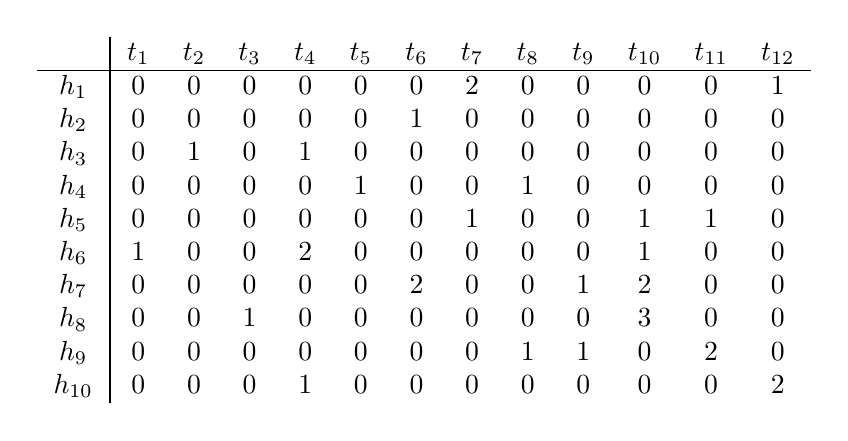
\begin{tikzpicture}[
    node distance=1cm,
    test/.style={circle, draw, thick, minimum size=0.6cm},
    decision/.style={circle, draw, thick, minimum size=0.55cm},
    leaf/.style={circle, draw, thick, fill=green!20, minimum size=0.5cm},
    arrow/.style={->, thick}
]

% Table of hypotheses vs tests (10 hypotheses, 12 tests, unbalanced outcomes)
\node[] at (0,0) {
\begin{tabular}{c|cccccccccccc}
 & $t_1$ & $t_2$ & $t_3$ & $t_4$ & $t_5$ & $t_6$ & $t_7$ & $t_8$ & $t_9$ & $t_{10}$ & $t_{11}$ & $t_{12}$ \\
\hline
$h_1$ & 0 & 0 & 0 & 0 & 0 & 0 & 2 & 0 & 0 & 0 & 0 & 1 \\
$h_2$ & 0 & 0 & 0 & 0 & 0 & 1 & 0 & 0 & 0 & 0 & 0 & 0 \\
$h_3$ & 0 & 1 & 0 & 1 & 0 & 0 & 0 & 0 & 0 & 0 & 0 & 0 \\
$h_4$ & 0 & 0 & 0 & 0 & 1 & 0 & 0 & 1 & 0 & 0 & 0 & 0 \\
$h_5$ & 0 & 0 & 0 & 0 & 0 & 0 & 1 & 0 & 0 & 1 & 1 & 0 \\
$h_6$ & 1 & 0 & 0 & 2 & 0 & 0 & 0 & 0 & 0 & 1 & 0 & 0 \\
$h_7$ & 0 & 0 & 0 & 0 & 0 & 2 & 0 & 0 & 1 & 2 & 0 & 0 \\
$h_8$ & 0 & 0 & 1 & 0 & 0 & 0 & 0 & 0 & 0 & 3 & 0 & 0 \\
$h_9$ & 0 & 0 & 0 & 0 & 0 & 0 & 0 & 1 & 1 & 0 & 2 & 0 \\
$h_{10}$ & 0 & 0 & 0 & 1 & 0 & 0 & 0 & 0 & 0 & 0 & 0 & 2 \\
\end{tabular}
};

\end{tikzpicture}
}
\normalsize
\caption*{(a) Hypotheses and tests table}
\end{minipage}

\begin{minipage}[t]{0.43\textwidth}
\centering
\scalebox{0.78}{
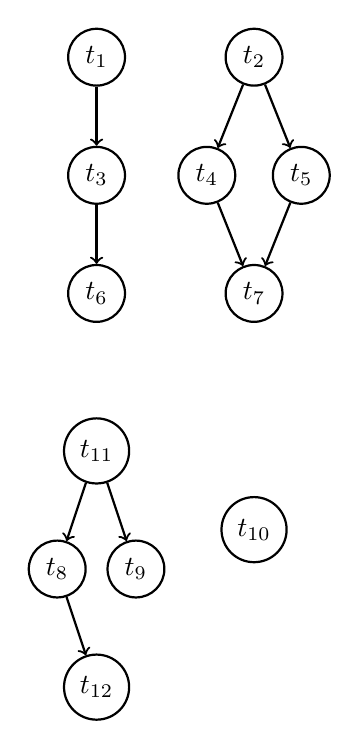
\begin{tikzpicture}[
    node distance=1cm,
    test/.style={circle, draw, thick, minimum size=0.6cm},
    arrow/.style={->, thick}
]

% DAG with 4 components (2 components on top, 2 below)
% Component 1 (top left)
\node[test] (t1) at (0.5,0) {$t_1$};
\node[test] (t3) at (0.5,-1.5) {$t_3$};
\node[test] (t6) at (0.5,-3) {$t_6$};
\draw[arrow] (t1) -- (t3);
\draw[arrow] (t3) -- (t6);

% Component 2 (top right)
\node[test] (t2) at (2.5,0) {$t_2$};
\node[test] (t4) at (1.9,-1.5) {$t_4$};
\node[test] (t5) at (3.1,-1.5) {$t_5$};
\node[test] (t7) at (2.5,-3) {$t_7$};
\draw[arrow] (t2) -- (t4);
\draw[arrow] (t2) -- (t5);
\draw[arrow] (t4) -- (t7);
\draw[arrow] (t5) -- (t7);

% Component 3 (bottom left)
\node[test] (t11) at (0.5,-5) {$t_{11}$};
\node[test] (t8) at (0,-6.5) {$t_8$};
\node[test] (t9) at (1,-6.5) {$t_9$};
\node[test] (t12) at (0.5,-8) {$t_{12}$};
\draw[arrow] (t11) -- (t8);
\draw[arrow] (t11) -- (t9);
\draw[arrow] (t8) -- (t12);

% Component 4 (isolated node, bottom right)
\node[test] (t10) at (2.5,-6) {$t_{10}$};

\end{tikzpicture}
}
\normalsize
\caption*{(b) Precedence}
\end{minipage}
\hfill
\begin{minipage}[t]{0.55\textwidth}
\centering
\scalebox{0.78}{
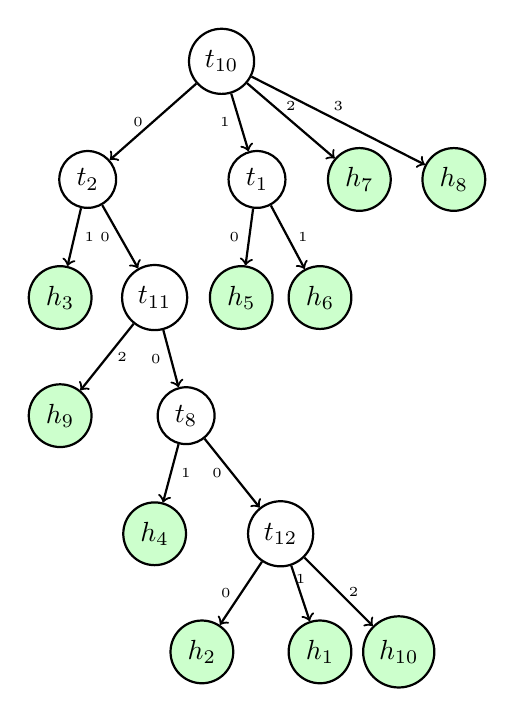
\begin{tikzpicture}[
    node distance=1cm,
    decision/.style={circle, draw, thick, minimum size=0.55cm},
    leaf/.style={circle, draw, thick, fill=green!20, minimum size=0.5cm},
    arrow/.style={->, thick}
]

% Decision tree built from table analysis
% Root: t10 (separates: h5→1, h6→1, h7→2, h8→3, rest→0)
\node[decision] (root) at (4.25,0) {$t_{10}$};

% t10=0: {h1,h2,h3,h4,h9,h10}
\node[decision] (n1) at (2.55,-1.5) {$t_2$};
% t10=1: {h5,h6}
\node[decision] (n2) at (4.7,-1.5) {$t_1$};
% t10=2: {h7}
\node[leaf] (h7) at (6,-1.5) {$h_7$};
% t10=3: {h8}
\node[leaf] (h8) at (7.2,-1.5) {$h_8$};

% t10=0, t2=0: {h1,h2,h4,h9,h10}
\node[decision] (n3) at (3.4,-3) {$t_{11}$};
% t10=0, t2=1: {h3}
\node[leaf] (h3) at (2.2,-3) {$h_3$};

% t10=1, t1=0: {h5}
\node[leaf] (h5) at (4.5,-3) {$h_5$};
% t10=1, t1=1: {h6}
\node[leaf] (h6) at (5.5,-3) {$h_6$};

% t10=0, t2=0, t11=0: {h1,h2,h4,h10}
\node[decision] (n4) at (3.8,-4.5) {$t_8$};
% t10=0, t2=0, t11=1: {h5} - but h5 already separated
% t10=0, t2=0, t11=2: {h9}
\node[leaf] (h9) at (2.2,-4.5) {$h_9$};

% t10=0, t2=0, t11=0, t8=0: {h1,h2,h10}
\node[decision] (n5) at (5,-6) {$t_{12}$};
% t10=0, t2=0, t11=0, t8=1: {h4}
\node[leaf] (h4) at (3.4,-6) {$h_4$};

% t10=0, t2=0, t11=0, t8=0, t12=0: {h2}
\node[leaf] (h2) at (4,-7.5) {$h_2$};
% t10=0, t2=0, t11=0, t8=0, t12=1: {h1}
\node[leaf] (h1) at (5.5,-7.5) {$h_1$};
% t10=0, t2=0, t11=0, t8=0, t12=2: {h10}
\node[leaf] (h10) at (6.5,-7.5) {$h_{10}$};

% Edges
\draw[arrow] (root) -- (n1) node[midway, left, font=\tiny] {0};
\draw[arrow] (root) -- (n2) node[midway, left, font=\tiny] {1};
\draw[arrow] (root) -- (h7) node[midway, above, font=\tiny] {2};
\draw[arrow] (root) -- (h8) node[midway, above, font=\tiny] {3};

\draw[arrow] (n1) -- (n3) node[midway, left, font=\tiny] {0};
\draw[arrow] (n1) -- (h3) node[midway, right, font=\tiny] {1};

\draw[arrow] (n2) -- (h5) node[midway, left, font=\tiny] {0};
\draw[arrow] (n2) -- (h6) node[midway, right, font=\tiny] {1};

\draw[arrow] (n3) -- (n4) node[midway, left, font=\tiny] {0};
\draw[arrow] (n3) -- (h9) node[midway, right, font=\tiny] {2};

\draw[arrow] (n4) -- (n5) node[midway, left, font=\tiny] {0};
\draw[arrow] (n4) -- (h4) node[midway, right, font=\tiny] {1};

\draw[arrow] (n5) -- (h2) node[midway, left, font=\tiny] {0};
\draw[arrow] (n5) -- (h1) node[midway, above, font=\tiny] {1};
\draw[arrow] (n5) -- (h10) node[midway, right, font=\tiny] {2};

\end{tikzpicture}
}
\normalsize
\caption*{(c) Valid decision tree}
\end{minipage}

\caption{Decision tree with precedence.}\label{fig:pcal_example}
\end{minipage}
\hfill
\begin{minipage}[t]{0.47\textwidth}
\centering

\begin{minipage}[t]{0.6\textwidth}
\centering
\scalebox{0.57}{
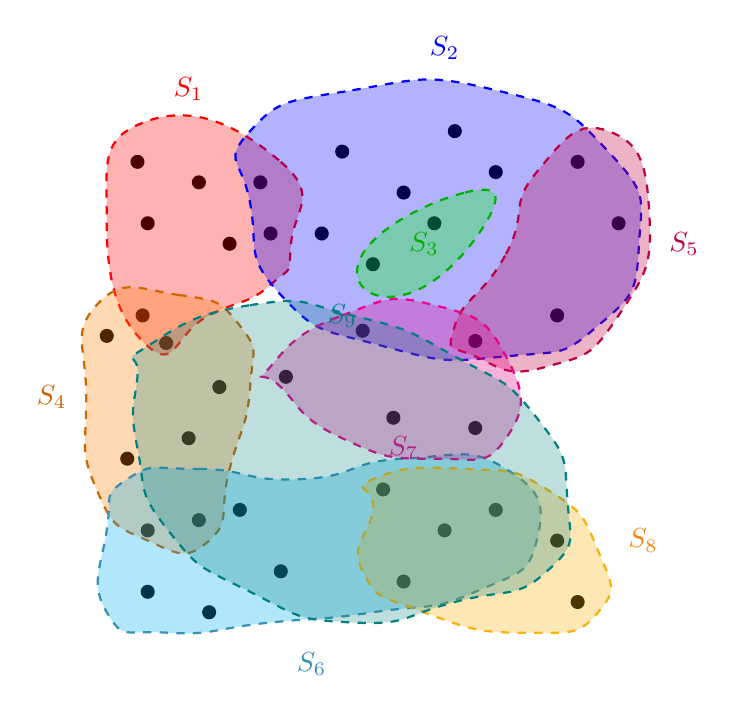
\begin{tikzpicture}[
    scale=1.3,
    node distance=1cm,
    element/.style={circle, draw, thick, fill=black, minimum size=0.15cm, inner sep=0pt},
    arrow/.style={->, thick}
]

% Universe elements - scattered randomly across the plane (35 elements with varied distribution)
\node[element] at (0.4, 3.9) {};
\node[element] at (0.9, 4.3) {};
\node[element] at (1.2, 3.7) {};
\node[element] at (0.35, 3) {};
\node[element] at (1.5, 4.3) {};
\node[element] at (0.3, 4.5) {};
\node[element] at (1.6, 3.8) {};  % SHARED by S1 and S2
\node[element] at (0.58, 2.73) {};  % SHARED by S1 and S4

\node[element] at (2.3, 4.6) {};
\node[element] at (2.9, 4.2) {};
\node[element] at (2.1, 3.8) {};
\node[element] at (3.4, 4.8) {};
\node[element] at (3.8, 4.4) {};
\node[element] at (2.6, 3.5) {};
\node[element] at (3.2, 3.9) {};

\node[element] at (4.6, 4.5) {};
\node[element] at (5, 3.9) {};
\node[element] at (4.4, 3) {};

\node[element] at (0, 2.8) {};
\node[element] at (1.1, 2.3) {};
\node[element] at (0.8, 1.8) {};
\node[element] at (0.2, 1.6) {};

\node[element] at (2.5, 2.85) {};
\node[element] at (3.6, 1.9) {};
\node[element] at (2.8, 2) {};
\node[element] at (3.6, 2.75) {};
\node[element] at (1.75, 2.4) {};

\node[element] at (0.9, 1.0) {};  % SHARED by S4 and S6
\node[element] at (0.4, 0.9) {};
\node[element] at (1.3, 1.1) {};
\node[element] at (0.4, 0.3) {};
\node[element] at (1.7, 0.5) {};
\node[element] at (1.0, 0.1) {};

\node[element] at (2.7, 1.3) {};
\node[element] at (3.3, 0.9) {};
\node[element] at (2.9, 0.4) {};
\node[element] at (3.8, 1.1) {};
\node[element] at (4.4, 0.8) {};
\node[element] at (4.6, 0.2) {};

% Set S1 (red) - includes (0.4,3.9) (0.9,4.3) (1.2,3.7) (0.6,3.2) (1.5,4.1) (0.3,4.5) + SHARED (1.6,4.0) (0.9,2.9)
\draw[thick, dashed, red, fill=red, fill opacity=0.3] 
    plot[smooth cycle, tension=1.0] coordinates {(0.4,4.9) (1.7,4.5) (1.8,3.7) (1.6,3.3) (1.0, 3) (0.4,2.7) (0.0,3.9)};
\node[above] at (0.8,5.0) {\textcolor{red}{$S_1$}};

% Set S2 (blue) - includes (2.3,4.6) (2.9,4.2) (2.1,3.8) (3.4,4.8) (3.8,4.4) (2.6,3.5) (3.2,3.9) (4.3,4.5) (4.7,3.9) (4.1,3.4) + SHARED (1.6,4.0)
\draw[thick, dashed, blue, fill=blue, fill opacity=0.3]
    plot[smooth cycle, tension=1.0] coordinates {(1.4,4.8) (2.4,5.2) (3.8,5.2) (4.9,4.6) (5.2,3.7) (4.8,2.9) (3.9,2.6) (2.7,2.7) (1.7,3.2) (1.4,4.1)};
\node[above] at (3.3,5.4) {\textcolor{blue}{$S_2$}};

% Set S3 (green) - small subset inside S2: (2.6,3.5) (3.2,3.9)
\draw[thick, dashed, green!70!black, fill=green, fill opacity=0.3]
    plot[smooth cycle, tension=1.0] coordinates {(2.5,3.6) (3.5,4.2) (3.7,3.9) (2.9,3.2)};
\node at (3.1,3.7) {\textcolor{green!70!black}{$S_3$}};

% Set S4 (orange) - includes (0.5,2.5) (1.1,2.8) (0.8,2.0) (0.2,1.6) + SHARED (0.9,1.0) (0.9,2.9)
\draw[thick, dashed, orange!80!black, fill=orange, fill opacity=0.3]
    plot[smooth cycle, tension=1.0] coordinates {(-0.1,3.1) (0.7,3.2) (1.3,2.9) (1.4,2.3) (1.2,1.5) (1.0,0.8) (0.4,0.8) (-0.1,1.3) (-0.2,2.2)};
\node[left] at (-0.3,2.2) {\textcolor{orange!80!black}{$S_4$}};

% Set S5 (purple) - right side elongated: (3.6,2.6) overlaps with S2 for (4.3,4.5) (4.7,3.9) (4.1,3.4)
\draw[thick, dashed, purple, fill=purple, fill opacity=0.3]
    plot[smooth cycle, tension=1.0] coordinates {(3.4,2.9) (3.9,3.6) (4.2,4.4) (4.9,4.8) (5.3,4.0) (5.0,3.0) (4.3,2.5) (3.6,2.6)};
\node[right] at (5.4,3.7) {\textcolor{purple}{$S_5$}};

% Set S6 (cyan) - includes (0.9,1.0) (0.7,0.8) (1.3,1.1) (0.4,0.3) (1.7,0.5) (1.0,0.1) (2.7,1.3) (3.3,0.9) (2.9,0.4) (3.8,1.1)
\draw[thick, dashed, cyan!70!black, fill=cyan, fill opacity=0.3]
    plot[smooth cycle, tension=1.0] coordinates {(0.2,1.4) (0.9,1.5) (1.9,1.4) (2.9,1.6) (3.9,1.5) (4.2,0.8) (3.6,0.3) (2.6,0.1) (1.6,0.0) (0.6,-0.1) (0.0,0.1) (0.0,0.9)};
\node[below] at (2.0,-0.2) {\textcolor{cyan!70!black}{$S_6$}};

% Set S7 (magenta) - includes (2.5,2.9) (3.1,2.4) (2.8,1.9) (1.9,2.2)
\draw[thick, dashed, magenta, fill=magenta, fill opacity=0.3]
    plot[smooth cycle, tension=1.0] coordinates {(1.6,2.5) (2.3,3.0) (3.2,3.1) (3.9,2.6) (3.9,1.8) (3.2,1.6) (2.3,1.8) (1.7,2.3)};
\node[above] at (2.9,1.5) {\textcolor{magenta}{$S_7$}};

% Set S8 (yellow!70!red) - includes (3.8,1.1) (4.4,0.6) (3.3,0.9) (2.9,0.4)
\draw[thick, dashed, yellow!70!red, fill=yellow!70!red, fill opacity=0.3]
    plot[smooth cycle, tension=1.0] coordinates {(2.6,1.4) (3.5,1.5) (4.3,1.3) (4.8,0.7) (4.8,0.1) (4.1,-0.1) (3.1,0.1) (2.5,0.5) (2.6,1.1)};
\node[right] at (5.0,0.8) {\textcolor{yellow!50!red}{$S_8$}};

% Set S9 (teal) - large blob filling gaps: overlaps with others to ensure complete coverage
\draw[thick, dashed, teal, fill=teal, fill opacity=0.25]
    plot[smooth cycle, tension=1.0] coordinates {(0.4,2.7) (1.4,3.1) (2.4,3.0) (3.4,2.6) (4.2,2.0) (4.5,1.2) (4.3,0.5) (3.4,0.2) (2.4,0.0) (1.4,0.3) (0.6,0.9) (0.3,1.7) (0.3,2.4)};
\node[below] at (2.3,3.2) {\textcolor{teal}{$S_9$}};

\end{tikzpicture}
}
\normalsize
\caption*{(a) Universe and sets}
\end{minipage}
\hfill
\begin{minipage}[t]{0.35\textwidth}
\centering
\scalebox{0.57}{
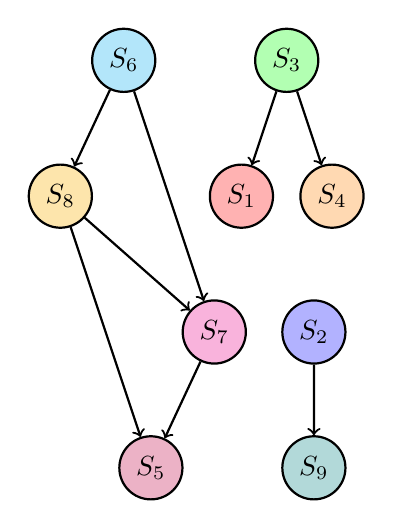
\begin{tikzpicture}[
    scale=1.15,
    node distance=1cm,
    set/.style={circle, draw, thick, minimum size=0.65cm},
    arrow/.style={->, thick}
]

% Precedence DAG with specified precedence constraints

% Component with S6 (left, wider)
\node[set, fill=cyan!30] (s6) at (0,0) {$S_6$};
\node[set, fill=yellow!70!red!30] (s8) at (-0.7,-1.5) {$S_8$};
\node[set, fill=magenta!30] (s7) at (1,-3) {$S_7$};
\node[set, fill=purple!30] (s5) at (0.3,-4.5) {$S_5$};

% Component with S3 (right top)
\node[set, fill=green!30] (s3) at (1.8,0) {$S_3$};
\node[set, fill=red!30] (s1) at (1.3,-1.5) {$S_1$};
\node[set, fill=orange!30] (s4) at (2.3,-1.5) {$S_4$};

% Component with S2 (right bottom)
\node[set, fill=blue!30] (s2) at (2.1,-3) {$S_2$};
\node[set, fill=teal!30] (s9) at (2.1,-4.5) {$S_9$};

% Precedence constraints (all arrows go down)
\draw[arrow] (s3) -- (s1);
\draw[arrow] (s3) -- (s4);
\draw[arrow] (s6) -- (s7);
\draw[arrow] (s6) -- (s8);
\draw[arrow] (s8) -- (s7);
\draw[arrow] (s8) -- (s5);
\draw[arrow] (s7) -- (s5);
\draw[arrow] (s2) -- (s9);

\end{tikzpicture}
}
\normalsize
\caption*{(b) Precedence}
\end{minipage}

\vspace{0.5cm}

\begin{minipage}[t]{\textwidth}
\centering
\scalebox{0.765}{
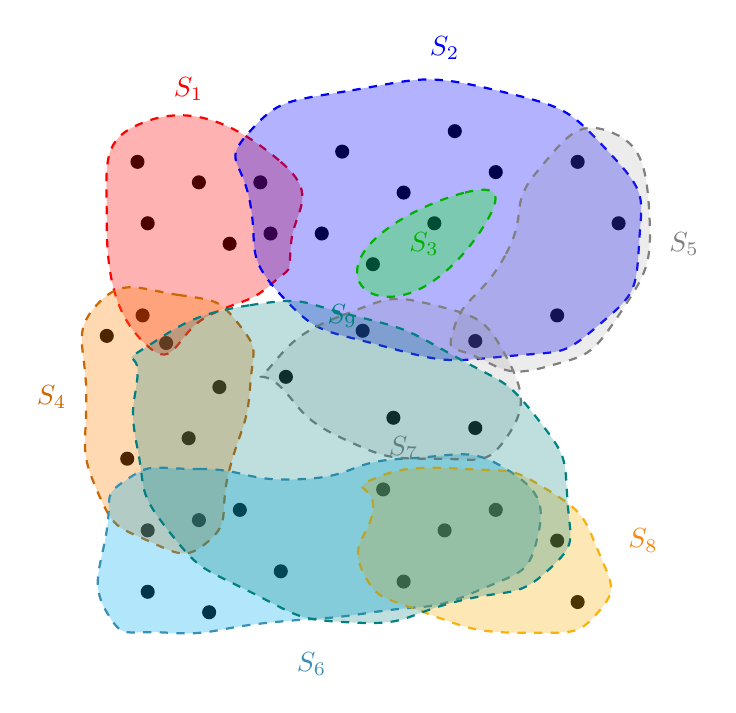
\begin{tikzpicture}[
    scale=1.3,
    node distance=1cm,
    element/.style={circle, draw, thick, fill=black, minimum size=0.15cm, inner sep=0pt},
    arrow/.style={->, thick}
]

% Universe elements - scattered randomly across the plane (35 elements with varied distribution)
\node[element] at (0.4, 3.9) {};
\node[element] at (0.9, 4.3) {};
\node[element] at (1.2, 3.7) {};
\node[element] at (0.35, 3) {};
\node[element] at (1.5, 4.3) {};
\node[element] at (0.3, 4.5) {};
\node[element] at (1.6, 3.8) {};  % SHARED by S1 and S2
\node[element] at (0.58, 2.73) {};  % SHARED by S1 and S4

\node[element] at (2.3, 4.6) {};
\node[element] at (2.9, 4.2) {};
\node[element] at (2.1, 3.8) {};
\node[element] at (3.4, 4.8) {};
\node[element] at (3.8, 4.4) {};
\node[element] at (2.6, 3.5) {};
\node[element] at (3.2, 3.9) {};

\node[element] at (4.6, 4.5) {};
\node[element] at (5, 3.9) {};
\node[element] at (4.4, 3) {};

\node[element] at (0, 2.8) {};
\node[element] at (1.1, 2.3) {};
\node[element] at (0.8, 1.8) {};
\node[element] at (0.2, 1.6) {};

\node[element] at (2.5, 2.85) {};
\node[element] at (3.6, 1.9) {};
\node[element] at (2.8, 2) {};
\node[element] at (3.6, 2.75) {};
\node[element] at (1.75, 2.4) {};

\node[element] at (0.9, 1.0) {};  % SHARED by S4 and S6
\node[element] at (0.4, 0.9) {};
\node[element] at (1.3, 1.1) {};
\node[element] at (0.4, 0.3) {};
\node[element] at (1.7, 0.5) {};
\node[element] at (1.0, 0.1) {};

\node[element] at (2.7, 1.3) {};
\node[element] at (3.3, 0.9) {};
\node[element] at (2.9, 0.4) {};
\node[element] at (3.8, 1.1) {};
\node[element] at (4.4, 0.8) {};
\node[element] at (4.6, 0.2) {};

% Set S1 (red) - SELECTED
\draw[thick, dashed, red, fill=red, fill opacity=0.3] 
    plot[smooth cycle, tension=1.0] coordinates {(0.4,4.9) (1.7,4.5) (1.8,3.7) (1.6,3.3) (1.0, 3) (0.4,2.7) (0.0,3.9)};
\node[above] at (0.8,5.0) {\textcolor{red}{\textbf{$S_1$}}};

% Set S2 (blue) - SELECTED
\draw[thick, dashed, blue, fill=blue, fill opacity=0.3]
    plot[smooth cycle, tension=1.0] coordinates {(1.4,4.8) (2.4,5.2) (3.8,5.2) (4.9,4.6) (5.2,3.7) (4.8,2.9) (3.9,2.6) (2.7,2.7) (1.7,3.2) (1.4,4.1)};
\node[above] at (3.3,5.4) {\textcolor{blue}{\textbf{$S_2$}}};

% Set S3 (green) - SELECTED
\draw[thick, dashed, green!70!black, fill=green, fill opacity=0.3]
    plot[smooth cycle, tension=1.0] coordinates {(2.5,3.6) (3.5,4.2) (3.7,3.9) (2.9,3.2)};
\node at (3.1,3.7) {\textcolor{green!70!black}{\textbf{$S_3$}}};

% Set S4 (orange) - SELECTED
\draw[thick, dashed, orange!80!black, fill=orange, fill opacity=0.3]
    plot[smooth cycle, tension=1.0] coordinates {(-0.1,3.1) (0.7,3.2) (1.3,2.9) (1.4,2.3) (1.2,1.5) (1.0,0.8) (0.4,0.8) (-0.1,1.3) (-0.2,2.2)};
\node[left] at (-0.3,2.2) {\textcolor{orange!80!black}{\textbf{$S_4$}}};

% Set S5 (purple) - NOT SELECTED (grayed out)
\draw[thick, dashed, gray, fill=gray, fill opacity=0.15]
    plot[smooth cycle, tension=1.0] coordinates {(3.4,2.9) (3.9,3.6) (4.2,4.4) (4.9,4.8) (5.3,4.0) (5.0,3.0) (4.3,2.5) (3.6,2.6)};
\node[right] at (5.4,3.7) {\textcolor{gray}{$S_5$}};

% Set S6 (cyan) - SELECTED
\draw[thick, dashed, cyan!70!black, fill=cyan, fill opacity=0.3]
    plot[smooth cycle, tension=1.0] coordinates {(0.2,1.4) (0.9,1.5) (1.9,1.4) (2.9,1.6) (3.9,1.5) (4.2,0.8) (3.6,0.3) (2.6,0.1) (1.6,0.0) (0.6,-0.1) (0.0,0.1) (0.0,0.9)};
\node[below] at (2.0,-0.2) {\textcolor{cyan!70!black}{\textbf{$S_6$}}};

% Set S7 (magenta) - NOT SELECTED (grayed out)
\draw[thick, dashed, gray, fill=gray, fill opacity=0.15]
    plot[smooth cycle, tension=1.0] coordinates {(1.6,2.5) (2.3,3.0) (3.2,3.1) (3.9,2.6) (3.9,1.8) (3.2,1.6) (2.3,1.8) (1.7,2.3)};
\node[above] at (2.9,1.5) {\textcolor{gray}{$S_7$}};

% Set S8 (yellow!70!red) - SELECTED
\draw[thick, dashed, yellow!70!red, fill=yellow!70!red, fill opacity=0.3]
    plot[smooth cycle, tension=1.0] coordinates {(2.6,1.4) (3.5,1.5) (4.3,1.3) (4.8,0.7) (4.8,0.1) (4.1,-0.1) (3.1,0.1) (2.5,0.5) (2.6,1.1)};
\node[right] at (5.0,0.8) {\textcolor{yellow!50!red}{\textbf{$S_8$}}};

% Set S9 (teal) - SELECTED
\draw[thick, dashed, teal, fill=teal, fill opacity=0.25]
    plot[smooth cycle, tension=1.0] coordinates {(0.4,2.7) (1.4,3.1) (2.4,3.0) (3.4,2.6) (4.2,2.0) (4.5,1.2) (4.3,0.5) (3.4,0.2) (2.4,0.0) (1.4,0.3) (0.6,0.9) (0.3,1.7) (0.3,2.4)};
\node[below] at (2.3,3.2) {\textcolor{teal}{\textbf{$S_9$}}};

\end{tikzpicture}
}
\normalsize
\caption*{(c) Solution: $\{S_1, S_2, S_6, S_8, S_9\}$ (in color)}
\end{minipage}


\caption{Set cover with precedence.}\label{fig:pccp_example}
\end{minipage}
\end{figure}

The aforementioned precedence constraints make the decision tree problem significantly more challenging. In a classical setup (without precedence constraints) the usual way of proceeding is to select at each step a test that maximizes some measure of information gain (e.g., reduction in entropy or number of remaining hypotheses). However, when precedence constraints are present, it may happen that the most informative test is not available at the current step, as some of its predecesors have not been performed yet. This requires more global planning and careful selection of tests to ensure that the decision tree remains valid with respect to the precedence constraints.
The method to address this issue is through a series of `reductions' between other optimization problems.
By this we mean an approach, where a particular algorithm for one problem uses an algorithm for another problem as a subroutine.
Particularly, we study a set covering problems with precedences:
We are given a set $\cU$ of $n$ items, a collection $\cS$ of $m$ subsets of $\cU$, such that $\bigcup_{S\in\cS}S=\cU$, an arbitrary partial order $(\cS,\preceq)$ on these subsets and a parameter $f$, $0<f<1$.
We say that a subfamily $\cC\subseteq\cS$ \emph{covers} at least $f$-fraction of items from $\cU$ if $\spr{\bigcup_{C\in\cC}C}\geq f\cdot n$.
We ask for a $\cC\subseteq\cS$ that covers at least $\f\cdot n$ items from $\cU$ and is \emph{precedence-closed}, that is, for each $x\in\cC$ and each $y\in\cS$ such that $y\preceq x$ it holds $y\in\cC$. We measure the quality of such $\cC$ by either its size $\spr{\cC}$ or the average time it takes to cover an item from $\cU$ (assuming some order of selecting sets from $\cC$ consistent with the precedence constraints). For a visual example of such a scenario consider Figure~\ref{fig:pccp_example}.
We show how to reduce the decision tree problem with precedences to the above set covering problems with precedences. Then we develop approximation algorithms for the set covering problems themselves. The approximation algorithms that we propose en route, e.g. for precedence constrained set cover, are of independent interest.

% \medskip
% \paraTitle{Outline.}
% In the next section we formally state all problems we address in this work.
% Section~\ref{sec:our-results} gives an overview of the main results of this work.
% Section~\ref{sec:AL} provides approximation algorithm for the above decision tree problem, assuming there exist certain approximations for variants of set cover.
% The latter are developed in Section~\ref{sec:SC}.
% Finally, set cover is solved via dense subfamily approximation from Section~\ref{sec:MDPCS}.
% The algorithms are supplemented with a number of inapproximability results in Section~\ref{sec:hardness}.

% Consider following problems:
% \begin{itemize}
%   \item  The \emph{Precedence Constrained Bayesian Decision Tree Problem} consists a set of $\mathcal{H}$ of $n$ hypothesis, a set $\cT$ of $m$ tests and a DAG (directed acyclic graph) $\mathcal{F} = \brc{\cT, \preceq}$ encoding the precedence constraints between available tests. Among $\mathcal{H}$ a hidden hypothesis is required to be encovered. To do so, the learner is allowed to perform tests, each of which reveals partial information about the hidden hypothesis. Upon receiving this information, the learner actively selects the next test to be performed. Importantly, in order to perform such test the learner needs to perform all of its predecesors in $\mathcal{F}$ first. The goal is to uncover the hidden hypothesis while performing as few tests as possible. Depending on the chosen criterion we distinguish between the \emph{Precedence Constrained Worst Case Decision Tree} (PCWCDT) and \emph{Precedence Constrained Average Case Decision Tree} (PCACDT) problems.
%   \item The \emph{Precedence Constrained Covering Problem} consists of a set of $n$ items $\mathcal{U}$, a collection $\mathcal{S}$ of $m$ subsets of $\mathcal{U}$ that cover these items, and a DAG $\mathcal{F} = \brc{\mathcal{S}, \preceq}$ encoding the precedence constraints between available subsets. The goal is to select a sequence of tests that covers at least $K$ items. Depending on the chosen criterion we distinguish between the \emph{Precedence Constrained Set Cover} (PCSC) and \emph{Precedence Constrained Min-Sum Set Cover} (PCMSSC) problems. In the first we are only interested in minimizing the number of selected subsets, while in the second we want to minimize the average time it takes to cover an item.
% \end{itemize}

\subsection{Problem formulations and outline} \label{sec:problems}



\subsection{Related Work}

\paragraph{Optimal Decision Tree}
Optimal decision tree is among the classical problems in computer science and has been studied extensively, starting with Garey \cite{GareyPerfBoundsOnSplittingAlgForBinTesting} in the 1970s. 
Since that time, it has gathered a lot of attention due to its numerous applications which include medical diagnosis, troubleshooting, active learning, and information retrieval. 
This problem is usually studied under two different optimization criteria: minimizing the worst-case cost and minimizing the average-case cost. 
Both versions of the problem are known to be NP-hard and cannot be approximated within an $o\br{\log n}$ factor \cite{ConstructOptimalBinaryDecisionTreesIsNPComplete,HardnessOfMinHeightDTP,ApproximatingDecisionTreesMultiwayBranches,DiagnosisDetermination}. Moreover, this bound is known to be tight and several $\cO(\log n)$-approximation algorithms for both non-uniform probabilities and cost average-case \cite{OptimalSplitTreeProblem,AnalysisGreedyActiveLearning,ApproximatingDecisionTreesMultiwayBranches,AverageCaseActiveLearningWithCosts,ApproximatingOptimalBinaryDecisionTrees,DTsforEntIdent,ApproxAlgsForOptDTsAndAdapTSPProblems,DiagnosisDetermination,AdaptiveSubmodularRankingAndRouting,AdaptivityInAdaptiveSubmodularity,MinimumCostAdaptiveSubmodularCover} as well as worst case \cite{DecisionTreesForGeometricModels,TheCostComplexityOfInteractiveLearning,DiagnosisDetermination}. Despite the hardness of the problem several special cases are known to have $o\br{\log n}$-approximation algorithms. For average case, this includes when tests have a constant number of possible outcomes and all probabilities and costs are uniform an $\cO\br{\log n/\log \log n}$-approximation is known \cite{TightAnalysisGreedyUniformDecisionTree}. This variant cannot be approximated within $\br{4-\epsilon}$ factor for any $\epsilon > 0$ unless P = NP \cite{DTsforEntIdent}. Moreover achieving any approximation factor above $9$ is not NP-hard assuming ETH \cite{TightAnalysisGreedyUniformDecisionTree}.
For worst case, when the underlying search space is a partially ordered set with a maximum element and costs are uniform an $\cO\br{\log n/\log \log n}$-approximation is known \cite{EdgeRankingSearchingPartialOrders}.


\paragraph{Searching in Trees}
For a special case when the instance represents searching in a tree, i.e., the set of hypothesis represents vertices of a tree and tests inform about the direction of the target placement with respect to the queried element (depending on the model, either vertices or edges can be queried), the problem has also been extensively studied. For uniform costs and worst-case criterion, a linear time exact algorithm is known for both edge query and vertex query variant \cite{Schaffer1989OptNodeRankOfTsInLinTime,OnakParys2006GenOfBSSInTsAndFLikePosets,Mozes_Onak2008FindOptTSStartInLinTime}. For average case, uniform costs and vertex queries an FPTAS is known \cite{SearchTreesOnGraphs}. For edge queries the problem is known to be NP-hard \cite{OnTheComplexityOfSearchingInTreesAverageCaseMinimization} and a greedy strategy achieves $3/2$-approximation \cite{TightApproximationBoundsOnASimpleAlgorithmForMinimumAverageSearchTimeInTrees}. For the case of non-uniform costs, the vertex query model generalizes edge query model. For worst case, the problem is known to be NP-hard \cite{EdgeRankingOfWeightedTrees,TheBinaryIdentificationProblemForWeightedTrees,OnTheTreeSearchProblemWithNonUniformCosts} and the best known approximation ratio is $\br{\sqrt{\log n}}$ \cite{ApproximationStrategiesforGeneralizedBinarySearchinWeightedTrees}.
The average case is also known to be NP-hard and an $\br{4+\epsilon}$-approximation FPTAS is known \cite{szyfelbein2025approximatingaveragecasegraphsearch}.

\paragraph{Set Cover with precedence constraints}

Set cover is the most important problem in combinatorial approximation algorithms.
It is well known that the greedy algorithm achieves an $H_n$-approximation for set cover \cite{GreedyHeuristicSetCoverProblem}, where $H_n=\cO\br{\log n}$ is the $n$-th harmonic number. Converesely, this is tight as set cover cannot be approximated within a $(1-\epsilon)\ln n$ factor for any $\epsilon > 0$ unless P=NP \cite{AnalyticalApproachToParallelRepetition}. The Min-Sum Set Cover is a version of the problem in which the goal is to minimize the average cover time of element. For this version, the greedy algorithm achieves $4$-approximation algorithm \cite{ApproximatingMinSumSetCover}, which is tight. When allowing arbitrary precedence constraints the problem admits an $\cO\br{\sqrt{m}}$-approximation algorithm and cannot be approximated within a $\cO\br{m^{1/6-\epsilon}}$ factor \cite{PCMSSC} subject to the Planted Dense Subgraph Conjecture \cite{OnApproxTargetSetSelection}.

\subsection{Our results and techniques} \label{sec:our-results}

Our main contribution consists of approximation algorithms and hardness results for decision tree and set covering problems with precedence constraints, studied under different structural restrictions on the precedence relation.

\paragraph{Approximation Results.} The key insight underlying our approach is a systematic hierarchy of reductions: we reduce decision tree problems to set covering problems with precedence constraints, which in turn are solved via algorithms for finding dense precedence-closed subfamilies. This hierarchy of reductions, illustrated in Figure~\ref{fig:reductions}, allows us to iteratively simplify the problem until we reach a core problem that can be effectively approximated. 
Our approximation results, including best known results from the literature, are summarized in Table~\ref{tab:results}

\begin{figure}[t!]
\centering
\begin{tikzpicture}[
    node distance=2.5cm and 3cm,
    problem/.style={rectangle, draw, very thick, minimum width=2.2cm, minimum height=1cm, align=center, font=\small},
    arrow/.style={->, very thick}
]

% Third row (define first for positioning)
\node[problem] (pcmssc) {PCMSSC};
\node[problem, right=3cm of pcmssc] (pcsc) {PCSC};

% Second row (above pcsc)
\node[problem, above right=0.7cm and 2cm of pcsc] (gst) {GST};

% Top row (above gst)
\node[problem, above left=0.6cm and 1.5cm of gst] (mdpcs) {MDPCS};

% Bottom row
\node[problem, below=0.6cm of pcmssc] (pcacal) {PCACAL};
\node[problem, below=0.6cm of pcsc] (pcwcal) {PCWCAL};
\node[problem, right=3cm of pcwcal] (pctc) {PCTC};

% Arrows
\draw[arrow] (mdpcs) -- (gst);
\draw[arrow] (mdpcs) -- (pcsc);
\draw[arrow] (mdpcs) -- (pcmssc);
\draw[arrow] (gst) -- (pcsc);
\draw[arrow] (pcsc) -- (pctc);
\draw[arrow] (pcsc) -- (pcwcal);
\draw[arrow] (pcmssc) -- (pcacal);

\end{tikzpicture}

\caption{Relationships between covering and decision tree problems, $\Pi_1 \to \Pi_2$ denotes that an approximation algorithm for problem $\Pi_1$ implies an approximation algorithm for problem $\Pi_2$.}\label{fig:reductions}
\end{figure}

\begin{table}[ht!]
\caption{Approximation guarantees for covering and decision tree problems under different precedence constraints. (* denotes new results, $H_n = \sum_{i=1}^{n} \frac{1}{i} = \Theta(\log n)$ is the $n$-th \emph{harmonic number}.).}
\label{tab:results}
\centering
{
\footnotesize
\begin{tabular}{p{0.077\linewidth}C{0.14\linewidth}C{0.14\linewidth}C{0.15\linewidth}C{0.13\linewidth}C{0.19\linewidth}}
\toprule
\textbf{prec.} & \textbf{\hyperref[problem:BPCSC]{B-PCSC}} & \textbf{\hyperref[problem:PCSC]{F-PCSC}} & \textbf{\hyperref[problem:PCMSSC]{F-PCMSSC}} & \textbf{\hyperref[problem:PCWCDT]{PCWCDT}} & \textbf{\hyperref[problem:PCACDT]{PCACDT}} \\
\midrule
\multirow{2}{\linewidth}{none} & $\br{1, \frac{e}{e-1}}$ & $\br{1, \frac{e}{e-1}}$  & $\br{\frac{4e}{e-1},1}$ & $\cO(\log n)$  & $\cO(\log n)$  \\
      &  \cite{TheBudgetedMaximumCoverageProblem} &  \cite{TheBudgetedMaximumCoverageProblem} & \cite{EfficientSequencesOfTrials} &  \cite{DiagnosisDetermination} & \cite{DiagnosisDetermination} \\

\addlinespace[2pt]
\cdashline{2-6}
\addlinespace[2pt]

inforest & $\br{1, \frac{e}{e-1}}$ (Thm.~\ref{thm:BPCSC-inforest}) & $\br{1, \frac{e}{e-1}}$ (Thm.~\ref{thm:BPCSC-inforest}) & $\br{3421.7, \frac{e}{e-1}}$ (Cor.~\ref{cor:BPCSC-inforest-to-PCMSSC})* & $\cO(\log n)$ (Cor.~\ref{cor:PCWCDT-special-cases})* & $\cO(\log(m+n))$ (Cor.~\ref{cor:PCACDT-special-cases})* \\


\addlinespace[2pt]
\cdashline{2-6}
\addlinespace[2pt]

outforest & $\br{\cO(\log n), 4}$ (Thm.~\ref{thm:BPCSC-outforest}) & $\br{\cO(\log n), 4}$ (Thm.~\ref{thm:BPCSC-outforest}) & $\br{\cO(\log n), 4}$ (Thm.~\ref{thm:BPCSC-outforest})* & $\cO(\log^2 n)$ (Cor.~\ref{cor:PCWCDT-special-cases})* & $\cO(\log^2(m+n))$ (Cor.~\ref{cor:PCACDT-special-cases})* \\


\addlinespace[2pt]
\cdashline{2-6}
\addlinespace[2pt]

general & $\br{\sqrt{m \cdot H_n}+1, 1}$ (Thm.~\ref{thm:BPCSC})* & $\br{\cO(\sqrt{m}/f), 2}$ (Thm.~\ref{thm:MDPCStoPCSC}), $\br{\sqrt{m \cdot H_n}+1, 1}$ (Cor.~\ref{cor:BPCSC-to-PCSC})* & $(\sqrt{m \cdot H_n}+1, 1)$ (Thm.~\ref{thm:BPCSC-to-PCMSSC})* & $\cO(\sqrt{m}\log n)$ (Thm.~\ref{thm:alphaPCWCDT})* & $\cO(\sqrt{m}\log^{3/2}\!(m+n))$ (Cor.~\ref{cor:PCACDT-special-cases})* \\
\bottomrule
\end{tabular}
}
\end{table}


For the most general case of arbitrary precedence constraints, we achieve $\cO(\sqrt{m}\log n)$-approximation for $\ProblemPCWCDT$ and $\cO(\sqrt{m}\log^{3/2}(m+n))$-approximation for $\ProblemPCACDT$, where $m$ is the number of tests and $n$ is the number of hypotheses. These results are obtained through a novel reduction to budgeted set cover problems ($\ProblemBPCSC$), for which we develop a $(\sqrt{m \cdot H_n}+1, 1)$-bicriteria approximation algorithm. The key technical innovation is an algorithm for the Max-Density Precedence-Closed Subfamily problem ($\ProblemMDPCS$), which iteratively selects precedence-closed subfamilies with high density (ratio of covered elements to subfamily size).

For the fractional set cover variant ($\ProblemPCSC$), we also provide a $(\cO(\sqrt{m}/f), 2)$-bicriteria approximation via $\ProblemMDPCS$, where $f$ is the target coverage fraction. For $\ProblemPCMSSC$, where the goal is to minimize the average coverage time, we develop an algorithm that converts any bicriteria approximation for $\ProblemBPCSC$ into an approximation for $\ProblemPCMSSC$. This reduction exploits a connection between coverage time and a careful partitioning of the budget parameter, yielding $(\sqrt{m \cdot H_n}+1, 1)$-approximation.

When the precedence constraints form special structures, we obtain significantly improved bounds. For outforests (where each element has at most one predecessor), we achieve $\cO(\log n)$-approximation for budgeted and fractional set cover by reducing to the Group Steiner Tree problem on trees. This translates to $\cO(\log^2 n)$-approximation for decision tree problems. For inforests (where each element has at most one successor), the problem admits constant-factor approximation: $(1, \frac{e}{e-1})$ for set cover problems, which we show via a careful analysis of a greedy algorithm that respects precedence constraints.

\paragraph{Hardness Results.} Our hardness results establish nearly matching lower bounds for most variants through a hierarchy of reductions illustrated in Figure~\ref{fig:hardness_diagram}. We systematically reduce from known hard problems such as Group Steiner Trees and Detecting Planted Dense Subgraphs to covering problems and then to decision tree problems, showing that achieving better approximation ratios is computationally hard even for special cases. Our hardness results, including best known results from the literature, are summarized in Table~\ref{tab:hardness}.

\begin{figure}[t!]
    \centering
    \begin{tikzpicture}[
    node distance=1.1cm and 2cm,
    problem/.style={rectangle, draw, very thick, minimum width=1.8cm, minimum height=0.8cm, align=center, font=\scriptsize},
    arrow/.style={->, very thick}
]

% Define positions based on the hand-drawn diagram
% Top level
\node[problem] (gst) at (-2, 0) {$\ProblemGST$};
\node[problem] (pds) at (2, 0) {$\ProblemPDS$};

% Middle level
\node[problem, below left=1.1cm and 0.5cm of pds] (fpcsc) {$\ProblemPCSC$};
\node[problem, below right=1.1cm and 0.5cm of pds] (fpcmssc) {$\ProblemPCMSSC$};

% Bottom level
\node[problem, below=1.1cm of fpcsc] (pcwcdt) {$\ProblemPCWCDT$};
\node[problem, below=1.1cm of fpcmssc] (pcacdt) {$\ProblemPCACDT$};

% Arrows with hyperlinks to sections
\draw[arrow] (gst) -- (fpcsc);
\draw[arrow] (pds) -- (fpcsc);
\draw[arrow] (pds) -- (fpcmssc);
\draw[arrow] (fpcsc) -- (pcwcdt);
\draw[arrow] (fpcsc) -- (pcacdt);
\draw[arrow] (fpcmssc) -- (pcacdt);

\end{tikzpicture}

    \caption{Inapproximability relations between problems, $\Pi_1 \to \Pi_2$ denotes that an inapproximability result for problem $\Pi_1$ implies an inapproximability result for problem $\Pi_2$.}
    \label{fig:hardness_diagram}
\end{figure}

\begin{table}[t!]
\caption{Hardness and inapproximability results for covering and decision tree problems. All results are from Section~\ref{sec:hardness}. PDS denotes results conditional on the Planted Dense Subgraph Conjecture. For general precedence constraints, $n$ denotes the universe size (or number of hypotheses) and $m$ denotes the number of sets (or tests).}
\label{tab:hardness}
\centering
{
\small
\begin{tabular}{lcccc}
\toprule
\textbf{prec} & \textbf{F-PCSC} & \textbf{PCMSSC} & \textbf{PCWCDT} & \textbf{PCACDT} \\
\midrule
none & $(1-o(1))H_n$ & $(4-\epsilon)$ & $o(\log n)$ & $o(\log n)$ \\
& \cite{AnalyticalApproachToParallelRepetition} & \cite{ApproximatingMinSumSetCover} & \cite{HardnessOfMinHeightDTP} & \cite{DTsforEntIdent} \\
\cdashline{2-5}
outforest & $o(\log^{2} n)$ & $o(\log^{2-\epsilon} n)$ & $o(\log^{2} n)$ & $o(\log^{2} n)$ \\
& (Thm.~\ref{thm:PCSC-outforest-hardness}) & \cite{ApproxAlgsForOptDTsAndAdapTSPProblems} & (Cor.~\ref{thm:PCWCDT-outforest-hardness}) & (Cor.~\ref{thm:PCACDT-outforest-hardness}) \\
\cdashline{2-5}
general & $o(n^{1/6})$, $o(m^{1/12})$ & $o(n^{1/6})$, $o(m^{1/12})$ & $o(n^{1/6})$, $o(m^{1/12})$ & $o(n^{1/6})$, $o(m^{1/12})$ \\
& (Thm.~\ref{thm:PCSC-PDS-hardness}) & (Thm.~\ref{thm:PCMSSC-PDS-hardness}) & (Cor.~\ref{thm:PCWCDT-PDS-hardness}) & (Cor.~\ref{thm:PCACDT-PDS-hardness}) \\
& PDS & PDS & PDS & PDS \\
\bottomrule
\end{tabular}
}
\end{table}


For arbitrary precedence constraints, we prove that under the Planted Dense Subgraph Conjecture, no algorithm can achieve $o(m^{1/6})$-approximation for $\ProblemPCSC$, $\ProblemPCMSSC$, $\ProblemPCWCDT$, or $\ProblemPCACDT$. This demonstrates a polynomial gap between our upper bounds and the hardness threshold. For outforest constraints, we establish $o(\log^2 n)$ hardness for $\ProblemPCSC$ by reducing from Group Steiner Tree on trees, which is known to be hard to approximate within $\cO(\log^2 n)$ unless $\text{NP}\subseteq \text{ZTIME}(n^{\text{polylog}(n)})$. This hardness naturally extends to decision tree problems via our reduction hierarchy.

Additionally, we show computational hardness for binary search with precedence constraints. Binary search on a path and search in tree-like partial orders are both special cases of decision tree problems where hypotheses correspond to vertices of a graph, and tests correspond to edge queries: each edge query partitions the hypotheses into two sets based on which side of the edge the target vertex lies. By reducing 3-SAT to binary search with precedence constraints on a path, we establish NP-hardness of the problem. Furthermore, we reduce Max-3-SAT to binary search in tree-like partial orders, obtaining APX-hardness. Note that both of these problems can be solved exactly in polynomial time without precedence constraints for the worst-case criterion and  average-case criterion, except for binary search in tree-like partial orders under average-case criterion, which is (weakly) NP-hard even without precedence constraints \cite{OnakParys2006GenOfBSSInTsAndFLikePosets}. Our problems are therefore belong to a rare class of problems which are hard even for the case of paths and untractable for trees.

% Our first theorem is due to Theorem~\ref{thm:alphaPCWCDT}.
% \begin{theorem} \label{thm:generalPCWCDT}
% There exists a polynomial-time $\bigo(\sqrt{m}\log n)$-approximation algorithm for the $\ProblemPCWCDT$, where $n$ is the number of hypotheses and $m$ is the number of tests.
% \end{theorem}
% Theorem~\ref{thm:alphaPCWCDT} relies on a bicriteria optimization algorithm for $\ProblemPCSC$ stated in Theorem~\ref{thm:MDPCStoPCSC} which in turn is obtained via an approximation algorithm for a problem called \emph{Max-Density Precedence-Closed Subfamily} ($\ProblemMDPCS$) given in \cite{PCMSSC}.
% \DD{(byc moze definicja MDPCS)}
% As a corollary of Theorem~\ref{thm:MDPCStoPCSC}, we obtain the following result regarding $\ProblemPCSC$.
% \begin{theorem} \label{thm:generalPCSC}
% There exists a polynomial-time $\bigo(\sqrt{m}f)$-approximation algorithm for $\ProblemPCSC$, where $m$ is the number of subsets over the universum of size $n$ and $f=k/n$, where $k$ is the required number of elements to be covered.
% \end{theorem}


% \begin{theorem} \label{thm:generalPCACDT}
% There exists a polynomial-time $\bigo(\sqrt{m}\log n)$-approximation algorithm for $\ProblemPCACDT$, where $m$ is the number of sets over the universum of size $n$.
% \end{theorem}

% \begin{theorem} \label{thm:generalPCMSSC}
% There exists a polynomial-time $\bigo(\sqrt{m})$-approximation algorithm for $\ProblemPCMSSC$, where $m$ is the number of sets over the universum.
% \end{theorem}



% \DD{Ten przykład jest super, ale chyba musimy znaleźć sposób na jego kompresję, tzn. nie stać nas na zapłacenie całej strony; około 1/3 strony byłaby ok (może tabelka obok drzewa decyzyjnego (moze zamiana kolumn vs wierszy aby ją powęzić, a może mocno zminimalizować przestrzeń między kolumnami, a partial order jako łuki pomiędzy etykietami wierszy tabelki?); też do przemyślenia gdzie ten przykład umieścić (raczej nie w ``contribution'', ale albo w intro, albo w preliminaries chyba}
% \begin{figure}[htb!]
% \centering
% \centering

\begin{minipage}[t]{\textwidth}
\centering
\scalebox{0.76}{
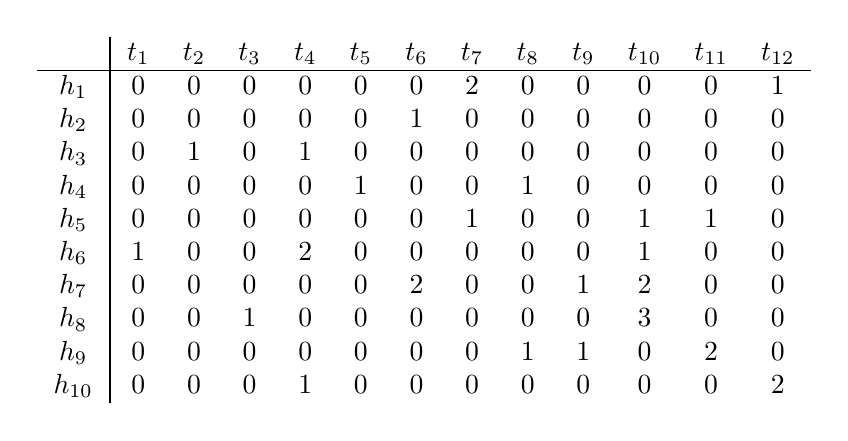
\begin{tikzpicture}[
    node distance=1cm,
    test/.style={circle, draw, thick, minimum size=0.6cm},
    decision/.style={circle, draw, thick, minimum size=0.55cm},
    leaf/.style={circle, draw, thick, fill=green!20, minimum size=0.5cm},
    arrow/.style={->, thick}
]

% Table of hypotheses vs tests (10 hypotheses, 12 tests, unbalanced outcomes)
\node[] at (0,0) {
\begin{tabular}{c|cccccccccccc}
 & $t_1$ & $t_2$ & $t_3$ & $t_4$ & $t_5$ & $t_6$ & $t_7$ & $t_8$ & $t_9$ & $t_{10}$ & $t_{11}$ & $t_{12}$ \\
\hline
$h_1$ & 0 & 0 & 0 & 0 & 0 & 0 & 2 & 0 & 0 & 0 & 0 & 1 \\
$h_2$ & 0 & 0 & 0 & 0 & 0 & 1 & 0 & 0 & 0 & 0 & 0 & 0 \\
$h_3$ & 0 & 1 & 0 & 1 & 0 & 0 & 0 & 0 & 0 & 0 & 0 & 0 \\
$h_4$ & 0 & 0 & 0 & 0 & 1 & 0 & 0 & 1 & 0 & 0 & 0 & 0 \\
$h_5$ & 0 & 0 & 0 & 0 & 0 & 0 & 1 & 0 & 0 & 1 & 1 & 0 \\
$h_6$ & 1 & 0 & 0 & 2 & 0 & 0 & 0 & 0 & 0 & 1 & 0 & 0 \\
$h_7$ & 0 & 0 & 0 & 0 & 0 & 2 & 0 & 0 & 1 & 2 & 0 & 0 \\
$h_8$ & 0 & 0 & 1 & 0 & 0 & 0 & 0 & 0 & 0 & 3 & 0 & 0 \\
$h_9$ & 0 & 0 & 0 & 0 & 0 & 0 & 0 & 1 & 1 & 0 & 2 & 0 \\
$h_{10}$ & 0 & 0 & 0 & 1 & 0 & 0 & 0 & 0 & 0 & 0 & 0 & 2 \\
\end{tabular}
};

\end{tikzpicture}
}
\normalsize
\caption*{(a) Hypotheses and tests table}
\end{minipage}

\begin{minipage}[t]{0.43\textwidth}
\centering
\scalebox{0.78}{
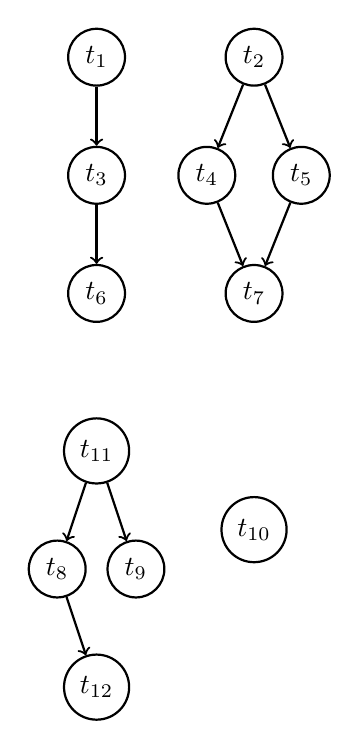
\begin{tikzpicture}[
    node distance=1cm,
    test/.style={circle, draw, thick, minimum size=0.6cm},
    arrow/.style={->, thick}
]

% DAG with 4 components (2 components on top, 2 below)
% Component 1 (top left)
\node[test] (t1) at (0.5,0) {$t_1$};
\node[test] (t3) at (0.5,-1.5) {$t_3$};
\node[test] (t6) at (0.5,-3) {$t_6$};
\draw[arrow] (t1) -- (t3);
\draw[arrow] (t3) -- (t6);

% Component 2 (top right)
\node[test] (t2) at (2.5,0) {$t_2$};
\node[test] (t4) at (1.9,-1.5) {$t_4$};
\node[test] (t5) at (3.1,-1.5) {$t_5$};
\node[test] (t7) at (2.5,-3) {$t_7$};
\draw[arrow] (t2) -- (t4);
\draw[arrow] (t2) -- (t5);
\draw[arrow] (t4) -- (t7);
\draw[arrow] (t5) -- (t7);

% Component 3 (bottom left)
\node[test] (t11) at (0.5,-5) {$t_{11}$};
\node[test] (t8) at (0,-6.5) {$t_8$};
\node[test] (t9) at (1,-6.5) {$t_9$};
\node[test] (t12) at (0.5,-8) {$t_{12}$};
\draw[arrow] (t11) -- (t8);
\draw[arrow] (t11) -- (t9);
\draw[arrow] (t8) -- (t12);

% Component 4 (isolated node, bottom right)
\node[test] (t10) at (2.5,-6) {$t_{10}$};

\end{tikzpicture}
}
\normalsize
\caption*{(b) Precedence}
\end{minipage}
\hfill
\begin{minipage}[t]{0.55\textwidth}
\centering
\scalebox{0.78}{
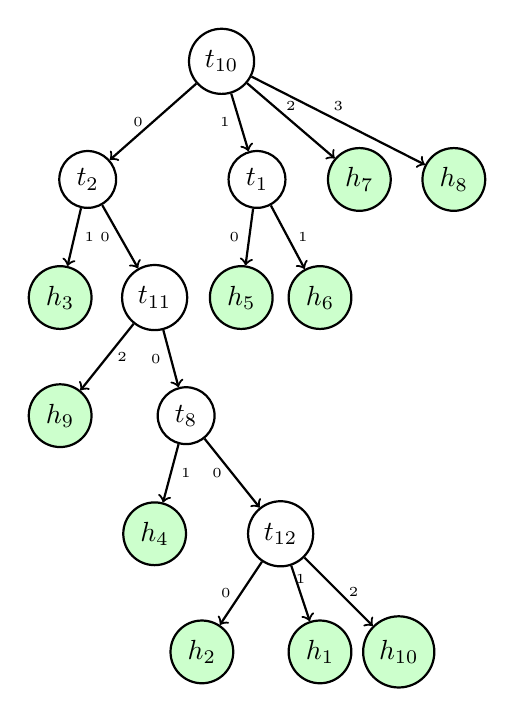
\begin{tikzpicture}[
    node distance=1cm,
    decision/.style={circle, draw, thick, minimum size=0.55cm},
    leaf/.style={circle, draw, thick, fill=green!20, minimum size=0.5cm},
    arrow/.style={->, thick}
]

% Decision tree built from table analysis
% Root: t10 (separates: h5→1, h6→1, h7→2, h8→3, rest→0)
\node[decision] (root) at (4.25,0) {$t_{10}$};

% t10=0: {h1,h2,h3,h4,h9,h10}
\node[decision] (n1) at (2.55,-1.5) {$t_2$};
% t10=1: {h5,h6}
\node[decision] (n2) at (4.7,-1.5) {$t_1$};
% t10=2: {h7}
\node[leaf] (h7) at (6,-1.5) {$h_7$};
% t10=3: {h8}
\node[leaf] (h8) at (7.2,-1.5) {$h_8$};

% t10=0, t2=0: {h1,h2,h4,h9,h10}
\node[decision] (n3) at (3.4,-3) {$t_{11}$};
% t10=0, t2=1: {h3}
\node[leaf] (h3) at (2.2,-3) {$h_3$};

% t10=1, t1=0: {h5}
\node[leaf] (h5) at (4.5,-3) {$h_5$};
% t10=1, t1=1: {h6}
\node[leaf] (h6) at (5.5,-3) {$h_6$};

% t10=0, t2=0, t11=0: {h1,h2,h4,h10}
\node[decision] (n4) at (3.8,-4.5) {$t_8$};
% t10=0, t2=0, t11=1: {h5} - but h5 already separated
% t10=0, t2=0, t11=2: {h9}
\node[leaf] (h9) at (2.2,-4.5) {$h_9$};

% t10=0, t2=0, t11=0, t8=0: {h1,h2,h10}
\node[decision] (n5) at (5,-6) {$t_{12}$};
% t10=0, t2=0, t11=0, t8=1: {h4}
\node[leaf] (h4) at (3.4,-6) {$h_4$};

% t10=0, t2=0, t11=0, t8=0, t12=0: {h2}
\node[leaf] (h2) at (4,-7.5) {$h_2$};
% t10=0, t2=0, t11=0, t8=0, t12=1: {h1}
\node[leaf] (h1) at (5.5,-7.5) {$h_1$};
% t10=0, t2=0, t11=0, t8=0, t12=2: {h10}
\node[leaf] (h10) at (6.5,-7.5) {$h_{10}$};

% Edges
\draw[arrow] (root) -- (n1) node[midway, left, font=\tiny] {0};
\draw[arrow] (root) -- (n2) node[midway, left, font=\tiny] {1};
\draw[arrow] (root) -- (h7) node[midway, above, font=\tiny] {2};
\draw[arrow] (root) -- (h8) node[midway, above, font=\tiny] {3};

\draw[arrow] (n1) -- (n3) node[midway, left, font=\tiny] {0};
\draw[arrow] (n1) -- (h3) node[midway, right, font=\tiny] {1};

\draw[arrow] (n2) -- (h5) node[midway, left, font=\tiny] {0};
\draw[arrow] (n2) -- (h6) node[midway, right, font=\tiny] {1};

\draw[arrow] (n3) -- (n4) node[midway, left, font=\tiny] {0};
\draw[arrow] (n3) -- (h9) node[midway, right, font=\tiny] {2};

\draw[arrow] (n4) -- (n5) node[midway, left, font=\tiny] {0};
\draw[arrow] (n4) -- (h4) node[midway, right, font=\tiny] {1};

\draw[arrow] (n5) -- (h2) node[midway, left, font=\tiny] {0};
\draw[arrow] (n5) -- (h1) node[midway, above, font=\tiny] {1};
\draw[arrow] (n5) -- (h10) node[midway, right, font=\tiny] {2};

\end{tikzpicture}
}
\normalsize
\caption*{(c) Valid decision tree}
\end{minipage}

% \caption{Example of a $\ProblemPCAL$ instance with 10 hypotheses and 12 tests. (a) Hypotheses-tests table. (b) Precedence DAG with four components. (c) A valid decision tree solution respecting precedence constraints.}\label{fig:pcal_example}
% \end{figure}
%
% \DD{na razie zakomentowałem rysunek dot zbiorów}
% \begin{figure}[h]
% \centering
% \centering

\begin{minipage}[t]{0.6\textwidth}
\centering
\scalebox{0.57}{
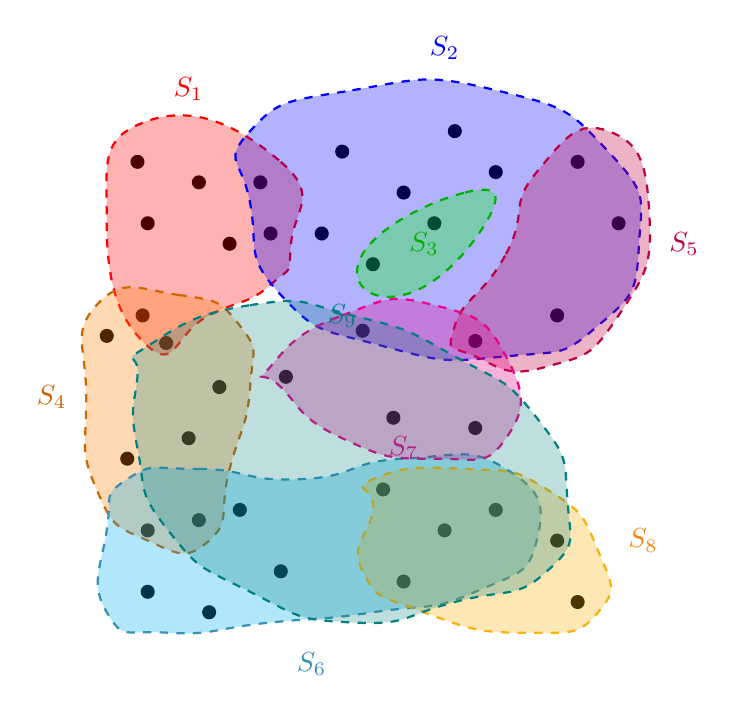
\begin{tikzpicture}[
    scale=1.3,
    node distance=1cm,
    element/.style={circle, draw, thick, fill=black, minimum size=0.15cm, inner sep=0pt},
    arrow/.style={->, thick}
]

% Universe elements - scattered randomly across the plane (35 elements with varied distribution)
\node[element] at (0.4, 3.9) {};
\node[element] at (0.9, 4.3) {};
\node[element] at (1.2, 3.7) {};
\node[element] at (0.35, 3) {};
\node[element] at (1.5, 4.3) {};
\node[element] at (0.3, 4.5) {};
\node[element] at (1.6, 3.8) {};  % SHARED by S1 and S2
\node[element] at (0.58, 2.73) {};  % SHARED by S1 and S4

\node[element] at (2.3, 4.6) {};
\node[element] at (2.9, 4.2) {};
\node[element] at (2.1, 3.8) {};
\node[element] at (3.4, 4.8) {};
\node[element] at (3.8, 4.4) {};
\node[element] at (2.6, 3.5) {};
\node[element] at (3.2, 3.9) {};

\node[element] at (4.6, 4.5) {};
\node[element] at (5, 3.9) {};
\node[element] at (4.4, 3) {};

\node[element] at (0, 2.8) {};
\node[element] at (1.1, 2.3) {};
\node[element] at (0.8, 1.8) {};
\node[element] at (0.2, 1.6) {};

\node[element] at (2.5, 2.85) {};
\node[element] at (3.6, 1.9) {};
\node[element] at (2.8, 2) {};
\node[element] at (3.6, 2.75) {};
\node[element] at (1.75, 2.4) {};

\node[element] at (0.9, 1.0) {};  % SHARED by S4 and S6
\node[element] at (0.4, 0.9) {};
\node[element] at (1.3, 1.1) {};
\node[element] at (0.4, 0.3) {};
\node[element] at (1.7, 0.5) {};
\node[element] at (1.0, 0.1) {};

\node[element] at (2.7, 1.3) {};
\node[element] at (3.3, 0.9) {};
\node[element] at (2.9, 0.4) {};
\node[element] at (3.8, 1.1) {};
\node[element] at (4.4, 0.8) {};
\node[element] at (4.6, 0.2) {};

% Set S1 (red) - includes (0.4,3.9) (0.9,4.3) (1.2,3.7) (0.6,3.2) (1.5,4.1) (0.3,4.5) + SHARED (1.6,4.0) (0.9,2.9)
\draw[thick, dashed, red, fill=red, fill opacity=0.3] 
    plot[smooth cycle, tension=1.0] coordinates {(0.4,4.9) (1.7,4.5) (1.8,3.7) (1.6,3.3) (1.0, 3) (0.4,2.7) (0.0,3.9)};
\node[above] at (0.8,5.0) {\textcolor{red}{$S_1$}};

% Set S2 (blue) - includes (2.3,4.6) (2.9,4.2) (2.1,3.8) (3.4,4.8) (3.8,4.4) (2.6,3.5) (3.2,3.9) (4.3,4.5) (4.7,3.9) (4.1,3.4) + SHARED (1.6,4.0)
\draw[thick, dashed, blue, fill=blue, fill opacity=0.3]
    plot[smooth cycle, tension=1.0] coordinates {(1.4,4.8) (2.4,5.2) (3.8,5.2) (4.9,4.6) (5.2,3.7) (4.8,2.9) (3.9,2.6) (2.7,2.7) (1.7,3.2) (1.4,4.1)};
\node[above] at (3.3,5.4) {\textcolor{blue}{$S_2$}};

% Set S3 (green) - small subset inside S2: (2.6,3.5) (3.2,3.9)
\draw[thick, dashed, green!70!black, fill=green, fill opacity=0.3]
    plot[smooth cycle, tension=1.0] coordinates {(2.5,3.6) (3.5,4.2) (3.7,3.9) (2.9,3.2)};
\node at (3.1,3.7) {\textcolor{green!70!black}{$S_3$}};

% Set S4 (orange) - includes (0.5,2.5) (1.1,2.8) (0.8,2.0) (0.2,1.6) + SHARED (0.9,1.0) (0.9,2.9)
\draw[thick, dashed, orange!80!black, fill=orange, fill opacity=0.3]
    plot[smooth cycle, tension=1.0] coordinates {(-0.1,3.1) (0.7,3.2) (1.3,2.9) (1.4,2.3) (1.2,1.5) (1.0,0.8) (0.4,0.8) (-0.1,1.3) (-0.2,2.2)};
\node[left] at (-0.3,2.2) {\textcolor{orange!80!black}{$S_4$}};

% Set S5 (purple) - right side elongated: (3.6,2.6) overlaps with S2 for (4.3,4.5) (4.7,3.9) (4.1,3.4)
\draw[thick, dashed, purple, fill=purple, fill opacity=0.3]
    plot[smooth cycle, tension=1.0] coordinates {(3.4,2.9) (3.9,3.6) (4.2,4.4) (4.9,4.8) (5.3,4.0) (5.0,3.0) (4.3,2.5) (3.6,2.6)};
\node[right] at (5.4,3.7) {\textcolor{purple}{$S_5$}};

% Set S6 (cyan) - includes (0.9,1.0) (0.7,0.8) (1.3,1.1) (0.4,0.3) (1.7,0.5) (1.0,0.1) (2.7,1.3) (3.3,0.9) (2.9,0.4) (3.8,1.1)
\draw[thick, dashed, cyan!70!black, fill=cyan, fill opacity=0.3]
    plot[smooth cycle, tension=1.0] coordinates {(0.2,1.4) (0.9,1.5) (1.9,1.4) (2.9,1.6) (3.9,1.5) (4.2,0.8) (3.6,0.3) (2.6,0.1) (1.6,0.0) (0.6,-0.1) (0.0,0.1) (0.0,0.9)};
\node[below] at (2.0,-0.2) {\textcolor{cyan!70!black}{$S_6$}};

% Set S7 (magenta) - includes (2.5,2.9) (3.1,2.4) (2.8,1.9) (1.9,2.2)
\draw[thick, dashed, magenta, fill=magenta, fill opacity=0.3]
    plot[smooth cycle, tension=1.0] coordinates {(1.6,2.5) (2.3,3.0) (3.2,3.1) (3.9,2.6) (3.9,1.8) (3.2,1.6) (2.3,1.8) (1.7,2.3)};
\node[above] at (2.9,1.5) {\textcolor{magenta}{$S_7$}};

% Set S8 (yellow!70!red) - includes (3.8,1.1) (4.4,0.6) (3.3,0.9) (2.9,0.4)
\draw[thick, dashed, yellow!70!red, fill=yellow!70!red, fill opacity=0.3]
    plot[smooth cycle, tension=1.0] coordinates {(2.6,1.4) (3.5,1.5) (4.3,1.3) (4.8,0.7) (4.8,0.1) (4.1,-0.1) (3.1,0.1) (2.5,0.5) (2.6,1.1)};
\node[right] at (5.0,0.8) {\textcolor{yellow!50!red}{$S_8$}};

% Set S9 (teal) - large blob filling gaps: overlaps with others to ensure complete coverage
\draw[thick, dashed, teal, fill=teal, fill opacity=0.25]
    plot[smooth cycle, tension=1.0] coordinates {(0.4,2.7) (1.4,3.1) (2.4,3.0) (3.4,2.6) (4.2,2.0) (4.5,1.2) (4.3,0.5) (3.4,0.2) (2.4,0.0) (1.4,0.3) (0.6,0.9) (0.3,1.7) (0.3,2.4)};
\node[below] at (2.3,3.2) {\textcolor{teal}{$S_9$}};

\end{tikzpicture}
}
\normalsize
\caption*{(a) Universe and sets}
\end{minipage}
\hfill
\begin{minipage}[t]{0.35\textwidth}
\centering
\scalebox{0.57}{
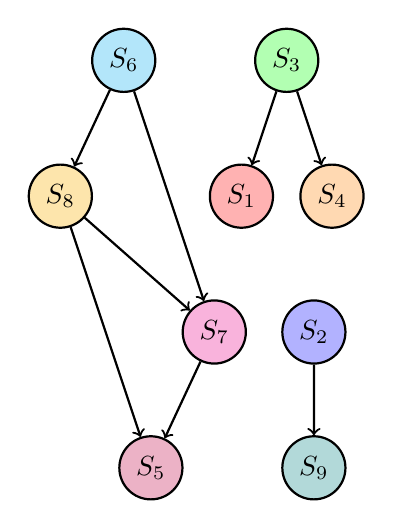
\begin{tikzpicture}[
    scale=1.15,
    node distance=1cm,
    set/.style={circle, draw, thick, minimum size=0.65cm},
    arrow/.style={->, thick}
]

% Precedence DAG with specified precedence constraints

% Component with S6 (left, wider)
\node[set, fill=cyan!30] (s6) at (0,0) {$S_6$};
\node[set, fill=yellow!70!red!30] (s8) at (-0.7,-1.5) {$S_8$};
\node[set, fill=magenta!30] (s7) at (1,-3) {$S_7$};
\node[set, fill=purple!30] (s5) at (0.3,-4.5) {$S_5$};

% Component with S3 (right top)
\node[set, fill=green!30] (s3) at (1.8,0) {$S_3$};
\node[set, fill=red!30] (s1) at (1.3,-1.5) {$S_1$};
\node[set, fill=orange!30] (s4) at (2.3,-1.5) {$S_4$};

% Component with S2 (right bottom)
\node[set, fill=blue!30] (s2) at (2.1,-3) {$S_2$};
\node[set, fill=teal!30] (s9) at (2.1,-4.5) {$S_9$};

% Precedence constraints (all arrows go down)
\draw[arrow] (s3) -- (s1);
\draw[arrow] (s3) -- (s4);
\draw[arrow] (s6) -- (s7);
\draw[arrow] (s6) -- (s8);
\draw[arrow] (s8) -- (s7);
\draw[arrow] (s8) -- (s5);
\draw[arrow] (s7) -- (s5);
\draw[arrow] (s2) -- (s9);

\end{tikzpicture}
}
\normalsize
\caption*{(b) Precedence}
\end{minipage}

\vspace{0.5cm}

\begin{minipage}[t]{\textwidth}
\centering
\scalebox{0.765}{
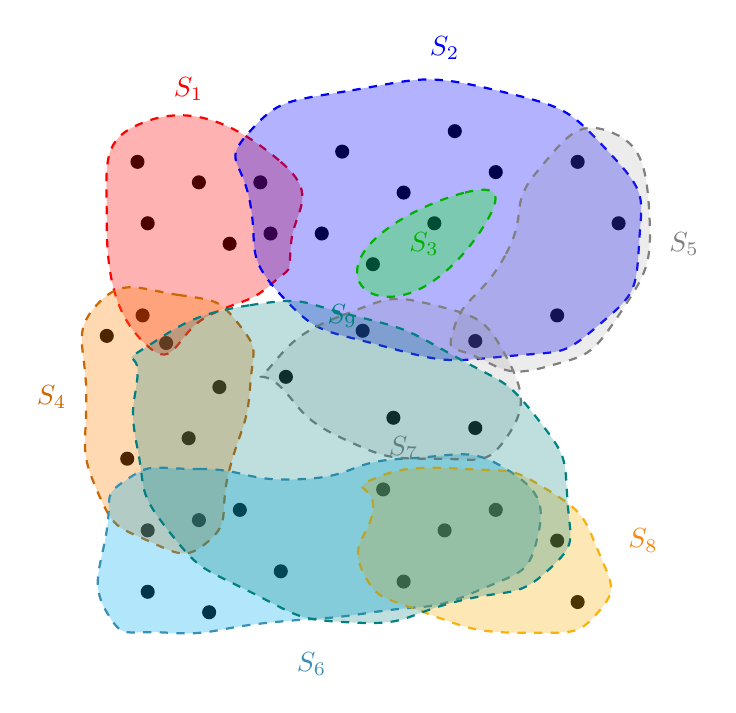
\begin{tikzpicture}[
    scale=1.3,
    node distance=1cm,
    element/.style={circle, draw, thick, fill=black, minimum size=0.15cm, inner sep=0pt},
    arrow/.style={->, thick}
]

% Universe elements - scattered randomly across the plane (35 elements with varied distribution)
\node[element] at (0.4, 3.9) {};
\node[element] at (0.9, 4.3) {};
\node[element] at (1.2, 3.7) {};
\node[element] at (0.35, 3) {};
\node[element] at (1.5, 4.3) {};
\node[element] at (0.3, 4.5) {};
\node[element] at (1.6, 3.8) {};  % SHARED by S1 and S2
\node[element] at (0.58, 2.73) {};  % SHARED by S1 and S4

\node[element] at (2.3, 4.6) {};
\node[element] at (2.9, 4.2) {};
\node[element] at (2.1, 3.8) {};
\node[element] at (3.4, 4.8) {};
\node[element] at (3.8, 4.4) {};
\node[element] at (2.6, 3.5) {};
\node[element] at (3.2, 3.9) {};

\node[element] at (4.6, 4.5) {};
\node[element] at (5, 3.9) {};
\node[element] at (4.4, 3) {};

\node[element] at (0, 2.8) {};
\node[element] at (1.1, 2.3) {};
\node[element] at (0.8, 1.8) {};
\node[element] at (0.2, 1.6) {};

\node[element] at (2.5, 2.85) {};
\node[element] at (3.6, 1.9) {};
\node[element] at (2.8, 2) {};
\node[element] at (3.6, 2.75) {};
\node[element] at (1.75, 2.4) {};

\node[element] at (0.9, 1.0) {};  % SHARED by S4 and S6
\node[element] at (0.4, 0.9) {};
\node[element] at (1.3, 1.1) {};
\node[element] at (0.4, 0.3) {};
\node[element] at (1.7, 0.5) {};
\node[element] at (1.0, 0.1) {};

\node[element] at (2.7, 1.3) {};
\node[element] at (3.3, 0.9) {};
\node[element] at (2.9, 0.4) {};
\node[element] at (3.8, 1.1) {};
\node[element] at (4.4, 0.8) {};
\node[element] at (4.6, 0.2) {};

% Set S1 (red) - SELECTED
\draw[thick, dashed, red, fill=red, fill opacity=0.3] 
    plot[smooth cycle, tension=1.0] coordinates {(0.4,4.9) (1.7,4.5) (1.8,3.7) (1.6,3.3) (1.0, 3) (0.4,2.7) (0.0,3.9)};
\node[above] at (0.8,5.0) {\textcolor{red}{\textbf{$S_1$}}};

% Set S2 (blue) - SELECTED
\draw[thick, dashed, blue, fill=blue, fill opacity=0.3]
    plot[smooth cycle, tension=1.0] coordinates {(1.4,4.8) (2.4,5.2) (3.8,5.2) (4.9,4.6) (5.2,3.7) (4.8,2.9) (3.9,2.6) (2.7,2.7) (1.7,3.2) (1.4,4.1)};
\node[above] at (3.3,5.4) {\textcolor{blue}{\textbf{$S_2$}}};

% Set S3 (green) - SELECTED
\draw[thick, dashed, green!70!black, fill=green, fill opacity=0.3]
    plot[smooth cycle, tension=1.0] coordinates {(2.5,3.6) (3.5,4.2) (3.7,3.9) (2.9,3.2)};
\node at (3.1,3.7) {\textcolor{green!70!black}{\textbf{$S_3$}}};

% Set S4 (orange) - SELECTED
\draw[thick, dashed, orange!80!black, fill=orange, fill opacity=0.3]
    plot[smooth cycle, tension=1.0] coordinates {(-0.1,3.1) (0.7,3.2) (1.3,2.9) (1.4,2.3) (1.2,1.5) (1.0,0.8) (0.4,0.8) (-0.1,1.3) (-0.2,2.2)};
\node[left] at (-0.3,2.2) {\textcolor{orange!80!black}{\textbf{$S_4$}}};

% Set S5 (purple) - NOT SELECTED (grayed out)
\draw[thick, dashed, gray, fill=gray, fill opacity=0.15]
    plot[smooth cycle, tension=1.0] coordinates {(3.4,2.9) (3.9,3.6) (4.2,4.4) (4.9,4.8) (5.3,4.0) (5.0,3.0) (4.3,2.5) (3.6,2.6)};
\node[right] at (5.4,3.7) {\textcolor{gray}{$S_5$}};

% Set S6 (cyan) - SELECTED
\draw[thick, dashed, cyan!70!black, fill=cyan, fill opacity=0.3]
    plot[smooth cycle, tension=1.0] coordinates {(0.2,1.4) (0.9,1.5) (1.9,1.4) (2.9,1.6) (3.9,1.5) (4.2,0.8) (3.6,0.3) (2.6,0.1) (1.6,0.0) (0.6,-0.1) (0.0,0.1) (0.0,0.9)};
\node[below] at (2.0,-0.2) {\textcolor{cyan!70!black}{\textbf{$S_6$}}};

% Set S7 (magenta) - NOT SELECTED (grayed out)
\draw[thick, dashed, gray, fill=gray, fill opacity=0.15]
    plot[smooth cycle, tension=1.0] coordinates {(1.6,2.5) (2.3,3.0) (3.2,3.1) (3.9,2.6) (3.9,1.8) (3.2,1.6) (2.3,1.8) (1.7,2.3)};
\node[above] at (2.9,1.5) {\textcolor{gray}{$S_7$}};

% Set S8 (yellow!70!red) - SELECTED
\draw[thick, dashed, yellow!70!red, fill=yellow!70!red, fill opacity=0.3]
    plot[smooth cycle, tension=1.0] coordinates {(2.6,1.4) (3.5,1.5) (4.3,1.3) (4.8,0.7) (4.8,0.1) (4.1,-0.1) (3.1,0.1) (2.5,0.5) (2.6,1.1)};
\node[right] at (5.0,0.8) {\textcolor{yellow!50!red}{\textbf{$S_8$}}};

% Set S9 (teal) - SELECTED
\draw[thick, dashed, teal, fill=teal, fill opacity=0.25]
    plot[smooth cycle, tension=1.0] coordinates {(0.4,2.7) (1.4,3.1) (2.4,3.0) (3.4,2.6) (4.2,2.0) (4.5,1.2) (4.3,0.5) (3.4,0.2) (2.4,0.0) (1.4,0.3) (0.6,0.9) (0.3,1.7) (0.3,2.4)};
\node[below] at (2.3,3.2) {\textcolor{teal}{\textbf{$S_9$}}};

\end{tikzpicture}
}
\normalsize
\caption*{(c) Solution: $\{S_1, S_2, S_6, S_8, S_9\}$ (in color)}
\end{minipage}


% \caption{Example of a PCCP instance with 39 elements and 9 covering sets. (a) Universe with covering sets. (b) Precedence DAG with three components. (c) Solution using 7 selected sets (colored).}\label{fig:pccp_example}
% \end{figure}

% \begin{figure}[h]
% \centering
% \centering

\begin{minipage}[t]{0.6\textwidth}
\centering
\scalebox{0.57}{
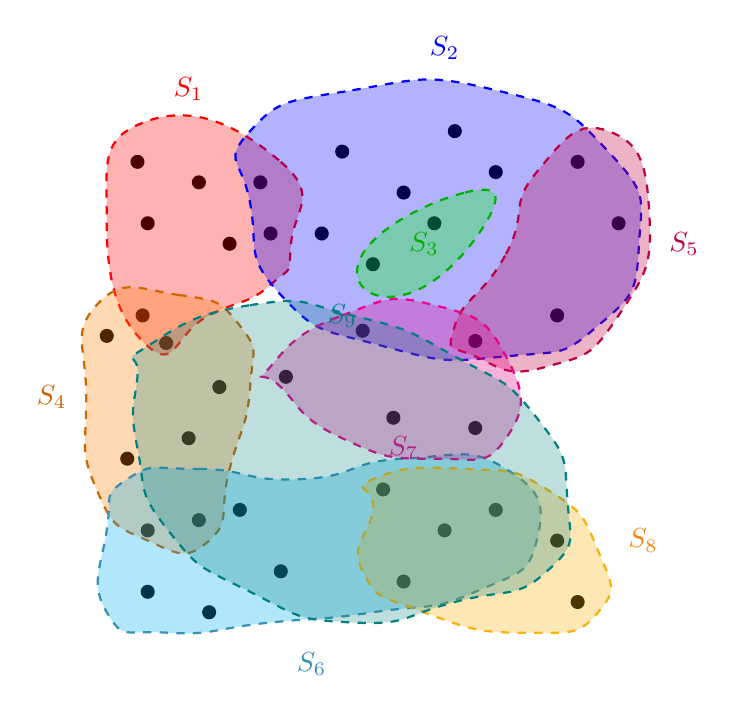
\begin{tikzpicture}[
    scale=1.3,
    node distance=1cm,
    element/.style={circle, draw, thick, fill=black, minimum size=0.15cm, inner sep=0pt},
    arrow/.style={->, thick}
]

% Universe elements - scattered randomly across the plane (35 elements with varied distribution)
\node[element] at (0.4, 3.9) {};
\node[element] at (0.9, 4.3) {};
\node[element] at (1.2, 3.7) {};
\node[element] at (0.35, 3) {};
\node[element] at (1.5, 4.3) {};
\node[element] at (0.3, 4.5) {};
\node[element] at (1.6, 3.8) {};  % SHARED by S1 and S2
\node[element] at (0.58, 2.73) {};  % SHARED by S1 and S4

\node[element] at (2.3, 4.6) {};
\node[element] at (2.9, 4.2) {};
\node[element] at (2.1, 3.8) {};
\node[element] at (3.4, 4.8) {};
\node[element] at (3.8, 4.4) {};
\node[element] at (2.6, 3.5) {};
\node[element] at (3.2, 3.9) {};

\node[element] at (4.6, 4.5) {};
\node[element] at (5, 3.9) {};
\node[element] at (4.4, 3) {};

\node[element] at (0, 2.8) {};
\node[element] at (1.1, 2.3) {};
\node[element] at (0.8, 1.8) {};
\node[element] at (0.2, 1.6) {};

\node[element] at (2.5, 2.85) {};
\node[element] at (3.6, 1.9) {};
\node[element] at (2.8, 2) {};
\node[element] at (3.6, 2.75) {};
\node[element] at (1.75, 2.4) {};

\node[element] at (0.9, 1.0) {};  % SHARED by S4 and S6
\node[element] at (0.4, 0.9) {};
\node[element] at (1.3, 1.1) {};
\node[element] at (0.4, 0.3) {};
\node[element] at (1.7, 0.5) {};
\node[element] at (1.0, 0.1) {};

\node[element] at (2.7, 1.3) {};
\node[element] at (3.3, 0.9) {};
\node[element] at (2.9, 0.4) {};
\node[element] at (3.8, 1.1) {};
\node[element] at (4.4, 0.8) {};
\node[element] at (4.6, 0.2) {};

% Set S1 (red) - includes (0.4,3.9) (0.9,4.3) (1.2,3.7) (0.6,3.2) (1.5,4.1) (0.3,4.5) + SHARED (1.6,4.0) (0.9,2.9)
\draw[thick, dashed, red, fill=red, fill opacity=0.3] 
    plot[smooth cycle, tension=1.0] coordinates {(0.4,4.9) (1.7,4.5) (1.8,3.7) (1.6,3.3) (1.0, 3) (0.4,2.7) (0.0,3.9)};
\node[above] at (0.8,5.0) {\textcolor{red}{$S_1$}};

% Set S2 (blue) - includes (2.3,4.6) (2.9,4.2) (2.1,3.8) (3.4,4.8) (3.8,4.4) (2.6,3.5) (3.2,3.9) (4.3,4.5) (4.7,3.9) (4.1,3.4) + SHARED (1.6,4.0)
\draw[thick, dashed, blue, fill=blue, fill opacity=0.3]
    plot[smooth cycle, tension=1.0] coordinates {(1.4,4.8) (2.4,5.2) (3.8,5.2) (4.9,4.6) (5.2,3.7) (4.8,2.9) (3.9,2.6) (2.7,2.7) (1.7,3.2) (1.4,4.1)};
\node[above] at (3.3,5.4) {\textcolor{blue}{$S_2$}};

% Set S3 (green) - small subset inside S2: (2.6,3.5) (3.2,3.9)
\draw[thick, dashed, green!70!black, fill=green, fill opacity=0.3]
    plot[smooth cycle, tension=1.0] coordinates {(2.5,3.6) (3.5,4.2) (3.7,3.9) (2.9,3.2)};
\node at (3.1,3.7) {\textcolor{green!70!black}{$S_3$}};

% Set S4 (orange) - includes (0.5,2.5) (1.1,2.8) (0.8,2.0) (0.2,1.6) + SHARED (0.9,1.0) (0.9,2.9)
\draw[thick, dashed, orange!80!black, fill=orange, fill opacity=0.3]
    plot[smooth cycle, tension=1.0] coordinates {(-0.1,3.1) (0.7,3.2) (1.3,2.9) (1.4,2.3) (1.2,1.5) (1.0,0.8) (0.4,0.8) (-0.1,1.3) (-0.2,2.2)};
\node[left] at (-0.3,2.2) {\textcolor{orange!80!black}{$S_4$}};

% Set S5 (purple) - right side elongated: (3.6,2.6) overlaps with S2 for (4.3,4.5) (4.7,3.9) (4.1,3.4)
\draw[thick, dashed, purple, fill=purple, fill opacity=0.3]
    plot[smooth cycle, tension=1.0] coordinates {(3.4,2.9) (3.9,3.6) (4.2,4.4) (4.9,4.8) (5.3,4.0) (5.0,3.0) (4.3,2.5) (3.6,2.6)};
\node[right] at (5.4,3.7) {\textcolor{purple}{$S_5$}};

% Set S6 (cyan) - includes (0.9,1.0) (0.7,0.8) (1.3,1.1) (0.4,0.3) (1.7,0.5) (1.0,0.1) (2.7,1.3) (3.3,0.9) (2.9,0.4) (3.8,1.1)
\draw[thick, dashed, cyan!70!black, fill=cyan, fill opacity=0.3]
    plot[smooth cycle, tension=1.0] coordinates {(0.2,1.4) (0.9,1.5) (1.9,1.4) (2.9,1.6) (3.9,1.5) (4.2,0.8) (3.6,0.3) (2.6,0.1) (1.6,0.0) (0.6,-0.1) (0.0,0.1) (0.0,0.9)};
\node[below] at (2.0,-0.2) {\textcolor{cyan!70!black}{$S_6$}};

% Set S7 (magenta) - includes (2.5,2.9) (3.1,2.4) (2.8,1.9) (1.9,2.2)
\draw[thick, dashed, magenta, fill=magenta, fill opacity=0.3]
    plot[smooth cycle, tension=1.0] coordinates {(1.6,2.5) (2.3,3.0) (3.2,3.1) (3.9,2.6) (3.9,1.8) (3.2,1.6) (2.3,1.8) (1.7,2.3)};
\node[above] at (2.9,1.5) {\textcolor{magenta}{$S_7$}};

% Set S8 (yellow!70!red) - includes (3.8,1.1) (4.4,0.6) (3.3,0.9) (2.9,0.4)
\draw[thick, dashed, yellow!70!red, fill=yellow!70!red, fill opacity=0.3]
    plot[smooth cycle, tension=1.0] coordinates {(2.6,1.4) (3.5,1.5) (4.3,1.3) (4.8,0.7) (4.8,0.1) (4.1,-0.1) (3.1,0.1) (2.5,0.5) (2.6,1.1)};
\node[right] at (5.0,0.8) {\textcolor{yellow!50!red}{$S_8$}};

% Set S9 (teal) - large blob filling gaps: overlaps with others to ensure complete coverage
\draw[thick, dashed, teal, fill=teal, fill opacity=0.25]
    plot[smooth cycle, tension=1.0] coordinates {(0.4,2.7) (1.4,3.1) (2.4,3.0) (3.4,2.6) (4.2,2.0) (4.5,1.2) (4.3,0.5) (3.4,0.2) (2.4,0.0) (1.4,0.3) (0.6,0.9) (0.3,1.7) (0.3,2.4)};
\node[below] at (2.3,3.2) {\textcolor{teal}{$S_9$}};

\end{tikzpicture}
}
\normalsize
\caption*{(a) Universe and sets}
\end{minipage}
\hfill
\begin{minipage}[t]{0.35\textwidth}
\centering
\scalebox{0.57}{
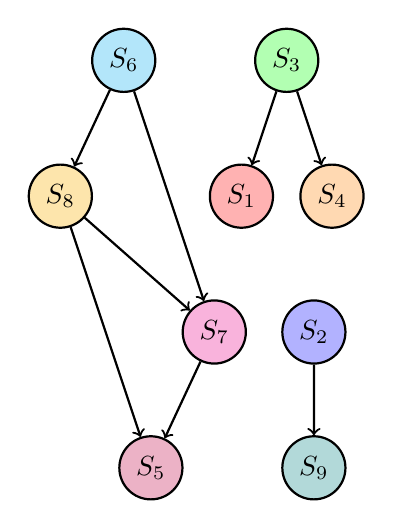
\begin{tikzpicture}[
    scale=1.15,
    node distance=1cm,
    set/.style={circle, draw, thick, minimum size=0.65cm},
    arrow/.style={->, thick}
]

% Precedence DAG with specified precedence constraints

% Component with S6 (left, wider)
\node[set, fill=cyan!30] (s6) at (0,0) {$S_6$};
\node[set, fill=yellow!70!red!30] (s8) at (-0.7,-1.5) {$S_8$};
\node[set, fill=magenta!30] (s7) at (1,-3) {$S_7$};
\node[set, fill=purple!30] (s5) at (0.3,-4.5) {$S_5$};

% Component with S3 (right top)
\node[set, fill=green!30] (s3) at (1.8,0) {$S_3$};
\node[set, fill=red!30] (s1) at (1.3,-1.5) {$S_1$};
\node[set, fill=orange!30] (s4) at (2.3,-1.5) {$S_4$};

% Component with S2 (right bottom)
\node[set, fill=blue!30] (s2) at (2.1,-3) {$S_2$};
\node[set, fill=teal!30] (s9) at (2.1,-4.5) {$S_9$};

% Precedence constraints (all arrows go down)
\draw[arrow] (s3) -- (s1);
\draw[arrow] (s3) -- (s4);
\draw[arrow] (s6) -- (s7);
\draw[arrow] (s6) -- (s8);
\draw[arrow] (s8) -- (s7);
\draw[arrow] (s8) -- (s5);
\draw[arrow] (s7) -- (s5);
\draw[arrow] (s2) -- (s9);

\end{tikzpicture}
}
\normalsize
\caption*{(b) Precedence}
\end{minipage}

\vspace{0.5cm}

\begin{minipage}[t]{\textwidth}
\centering
\scalebox{0.765}{
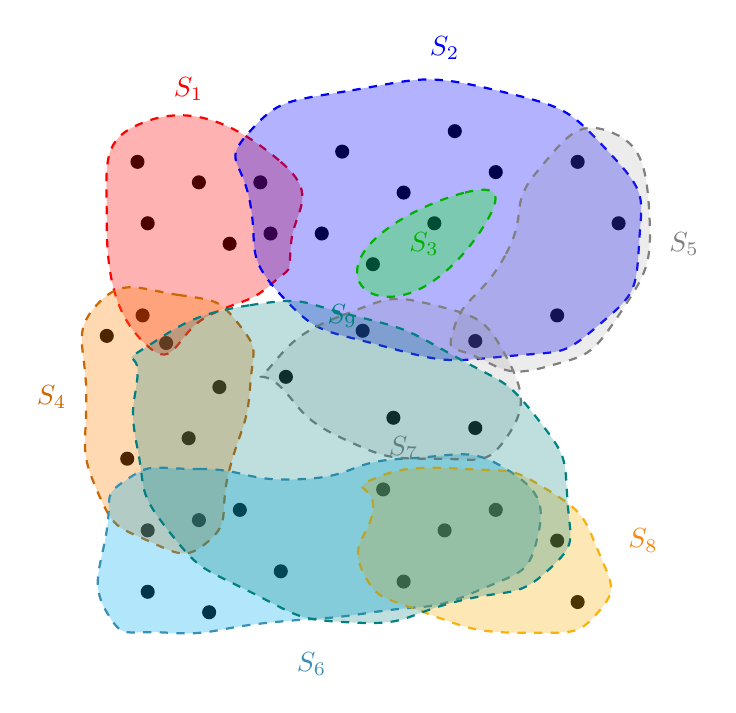
\begin{tikzpicture}[
    scale=1.3,
    node distance=1cm,
    element/.style={circle, draw, thick, fill=black, minimum size=0.15cm, inner sep=0pt},
    arrow/.style={->, thick}
]

% Universe elements - scattered randomly across the plane (35 elements with varied distribution)
\node[element] at (0.4, 3.9) {};
\node[element] at (0.9, 4.3) {};
\node[element] at (1.2, 3.7) {};
\node[element] at (0.35, 3) {};
\node[element] at (1.5, 4.3) {};
\node[element] at (0.3, 4.5) {};
\node[element] at (1.6, 3.8) {};  % SHARED by S1 and S2
\node[element] at (0.58, 2.73) {};  % SHARED by S1 and S4

\node[element] at (2.3, 4.6) {};
\node[element] at (2.9, 4.2) {};
\node[element] at (2.1, 3.8) {};
\node[element] at (3.4, 4.8) {};
\node[element] at (3.8, 4.4) {};
\node[element] at (2.6, 3.5) {};
\node[element] at (3.2, 3.9) {};

\node[element] at (4.6, 4.5) {};
\node[element] at (5, 3.9) {};
\node[element] at (4.4, 3) {};

\node[element] at (0, 2.8) {};
\node[element] at (1.1, 2.3) {};
\node[element] at (0.8, 1.8) {};
\node[element] at (0.2, 1.6) {};

\node[element] at (2.5, 2.85) {};
\node[element] at (3.6, 1.9) {};
\node[element] at (2.8, 2) {};
\node[element] at (3.6, 2.75) {};
\node[element] at (1.75, 2.4) {};

\node[element] at (0.9, 1.0) {};  % SHARED by S4 and S6
\node[element] at (0.4, 0.9) {};
\node[element] at (1.3, 1.1) {};
\node[element] at (0.4, 0.3) {};
\node[element] at (1.7, 0.5) {};
\node[element] at (1.0, 0.1) {};

\node[element] at (2.7, 1.3) {};
\node[element] at (3.3, 0.9) {};
\node[element] at (2.9, 0.4) {};
\node[element] at (3.8, 1.1) {};
\node[element] at (4.4, 0.8) {};
\node[element] at (4.6, 0.2) {};

% Set S1 (red) - SELECTED
\draw[thick, dashed, red, fill=red, fill opacity=0.3] 
    plot[smooth cycle, tension=1.0] coordinates {(0.4,4.9) (1.7,4.5) (1.8,3.7) (1.6,3.3) (1.0, 3) (0.4,2.7) (0.0,3.9)};
\node[above] at (0.8,5.0) {\textcolor{red}{\textbf{$S_1$}}};

% Set S2 (blue) - SELECTED
\draw[thick, dashed, blue, fill=blue, fill opacity=0.3]
    plot[smooth cycle, tension=1.0] coordinates {(1.4,4.8) (2.4,5.2) (3.8,5.2) (4.9,4.6) (5.2,3.7) (4.8,2.9) (3.9,2.6) (2.7,2.7) (1.7,3.2) (1.4,4.1)};
\node[above] at (3.3,5.4) {\textcolor{blue}{\textbf{$S_2$}}};

% Set S3 (green) - SELECTED
\draw[thick, dashed, green!70!black, fill=green, fill opacity=0.3]
    plot[smooth cycle, tension=1.0] coordinates {(2.5,3.6) (3.5,4.2) (3.7,3.9) (2.9,3.2)};
\node at (3.1,3.7) {\textcolor{green!70!black}{\textbf{$S_3$}}};

% Set S4 (orange) - SELECTED
\draw[thick, dashed, orange!80!black, fill=orange, fill opacity=0.3]
    plot[smooth cycle, tension=1.0] coordinates {(-0.1,3.1) (0.7,3.2) (1.3,2.9) (1.4,2.3) (1.2,1.5) (1.0,0.8) (0.4,0.8) (-0.1,1.3) (-0.2,2.2)};
\node[left] at (-0.3,2.2) {\textcolor{orange!80!black}{\textbf{$S_4$}}};

% Set S5 (purple) - NOT SELECTED (grayed out)
\draw[thick, dashed, gray, fill=gray, fill opacity=0.15]
    plot[smooth cycle, tension=1.0] coordinates {(3.4,2.9) (3.9,3.6) (4.2,4.4) (4.9,4.8) (5.3,4.0) (5.0,3.0) (4.3,2.5) (3.6,2.6)};
\node[right] at (5.4,3.7) {\textcolor{gray}{$S_5$}};

% Set S6 (cyan) - SELECTED
\draw[thick, dashed, cyan!70!black, fill=cyan, fill opacity=0.3]
    plot[smooth cycle, tension=1.0] coordinates {(0.2,1.4) (0.9,1.5) (1.9,1.4) (2.9,1.6) (3.9,1.5) (4.2,0.8) (3.6,0.3) (2.6,0.1) (1.6,0.0) (0.6,-0.1) (0.0,0.1) (0.0,0.9)};
\node[below] at (2.0,-0.2) {\textcolor{cyan!70!black}{\textbf{$S_6$}}};

% Set S7 (magenta) - NOT SELECTED (grayed out)
\draw[thick, dashed, gray, fill=gray, fill opacity=0.15]
    plot[smooth cycle, tension=1.0] coordinates {(1.6,2.5) (2.3,3.0) (3.2,3.1) (3.9,2.6) (3.9,1.8) (3.2,1.6) (2.3,1.8) (1.7,2.3)};
\node[above] at (2.9,1.5) {\textcolor{gray}{$S_7$}};

% Set S8 (yellow!70!red) - SELECTED
\draw[thick, dashed, yellow!70!red, fill=yellow!70!red, fill opacity=0.3]
    plot[smooth cycle, tension=1.0] coordinates {(2.6,1.4) (3.5,1.5) (4.3,1.3) (4.8,0.7) (4.8,0.1) (4.1,-0.1) (3.1,0.1) (2.5,0.5) (2.6,1.1)};
\node[right] at (5.0,0.8) {\textcolor{yellow!50!red}{\textbf{$S_8$}}};

% Set S9 (teal) - SELECTED
\draw[thick, dashed, teal, fill=teal, fill opacity=0.25]
    plot[smooth cycle, tension=1.0] coordinates {(0.4,2.7) (1.4,3.1) (2.4,3.0) (3.4,2.6) (4.2,2.0) (4.5,1.2) (4.3,0.5) (3.4,0.2) (2.4,0.0) (1.4,0.3) (0.6,0.9) (0.3,1.7) (0.3,2.4)};
\node[below] at (2.3,3.2) {\textcolor{teal}{\textbf{$S_9$}}};

\end{tikzpicture}
}
\normalsize
\caption*{(c) Solution: $\{S_1, S_2, S_6, S_8, S_9\}$ (in color)}
\end{minipage}


% \caption{Example of a PCCP instance with 39 elements and 9 covering sets. (a) Universe with covering sets. (b) Precedence DAG with three components. (c) Solution using 7 selected sets (colored).}\label{fig:pccp_example}
% \end{figure}

\DD{tutaj bylby jakis wywod i intuicje jakie techniki sa nowe, generalnie trzebaby sie pochwalic pomyslami roznymi}

\subsection{Organization}